\documentclass[12pt,
article,
type=sta, %sta, diplom, bsc, pp, msc, dr, drfinal, sem, prosem
colorbacktitle,
instlogo,
accentcolor=tud1c,
twoside
]{tudthesis}

\usepackage[ngerman]{babel}
%\usepackage[english]{babel}

\usepackage[latin1]{inputenc}
%\usepackage[applemac]{inputenc}

% linebreak for urls in bitex
\usepackage{url}
\urlstyle{rm}

%listings
\usepackage{listings}

% needed packages for ctrl
\usepackage{tikz}
\usepackage{pgfplots} 
\usepackage{pgfgantt}
\usepackage{pdflscape}
\pgfplotsset{compat=newest} 
\pgfplotsset{plot coordinates/math parser=false}
\usepackage{amsmath}
\usepackage{textcomp}
\usepackage{booktabs}
\usepackage{hyperref}

\newcommand{\getmydate}{%
\iflanguage{ngerman}{%
  \ifcase\month%
    \or Januar\or Februar\or M\"arz%
    \or April\or Mai\or Juni\or Juli%
    \or August\or September\or Oktober%
    \or November\or Dezember%
  \fi\ \number\year%
}%
\iflanguage{english}{%
  \ifcase\month%
    \or January\or February\or March%
    \or April\or May\or June\or July%
    \or August\or September\or October%
    \or November\or December%
  \fi\ \number\year%
}
}
% changed counter for section wise counting
\usepackage{chngcntr}
\counterwithin{figure}{section} 
\counterwithin{table}{section} 

 
\setinstitutionlogo[height]{logo/ESlogo.png}

\begin{document}
	\counterwithin{lstlisting}{section}
  \thesistitle{Projektseminar Echtzeitsysteme}%
    {Ausarbeitung}
  \author{The Fast and The Curious}
  %do not add your student id!
  %\studentidx{1145456}

  \referee{Stefan Tomaszek}{Stefan Tomaszek}
	
  \iflanguage{english}{
		\department{	\mbox{Department of Electrical Engineering}\\ and Information Technology (FB18)\\\\Adjunct Member Department of\\ Computer Science (FB20)\\\\Prof. Dr. rer. nat. A. Sch�rr\\\ Merckstra�e 25\\64283 Darmstadt\\\\www.es.tu-darmstadt.de}
		\group{Real-Time Systems Lab}
	}{
		\department{Elektrotechnik und \\Informationstechnik (FB18)\\\\Zweitmitglied Informatik (FB20)\\\\Prof. Dr. rer. nat. A. Sch�rr\\\ Merckstra�e 25\\64283 Darmstadt\\\\www.es.tu-darmstadt.de}
		\group{Fachgebiet Echtzeitsysteme}
	}
  
  \dateofsubmit{\today}
  \makethesistitle
  %\affidavit{Daniel Otterbach}
  %\affidavit{Daniel Pech}
  %\affidavit{Frederic Jacob}
  %\affidavit{Jens Balze}
  %\affidavit{Nils Hamacher}
	


	\pagenumbering{roman}
	\addtocontents{Anhang}{}
	\tableofcontents
	\cleardoublepage
	\listoffigures
	\cleardoublepage
	\listoftables
	\cleardoublepage
	
	\pagenumbering{arabic}
	\newcommand{\MATLAB}{\textsc{Matlab}\xspace}
	\section{Einleitung}
Das Projektseminar Echtzeitsysteme bietet Studenten die M\"oglichkeit echtzeitkritische Software mithilfe eines Roboterautos zu entwickeln. Dabei standen im Wintersemester 2018/2019 autonome Fahrassistenzsysteme im Vordergrund. In diesem Kapitel soll die Aufgabenstellung und die individuelle Themenwahl des Teams erl\"autert werden und ein \"Uberblick \"uber das gesamte Projekt geschaffen werden.

\subsection{Aufgabenstellung}
Die Aufgabenstellung des Projektseminars Echtzeitsysteme 2018/2019 setzte sich aus zwei Teilen zusammen. \\\\
Der erste, verpflichtende Teil stellte die Aufgabe dar, das Roboterauto selbstst\"andig eine Runde in einem vorgegebenen Rundkurs fahren zu lassen. Dabei wurden den Gruppen sowohl eine Kinect mit Farb- und Tiefenkamera, als auch eine Weitwinkel-Webcam zur Verf\"ugung gestellt. Es wurden Fahrbahnmarkierungen mit grellen Farben benutzt, um die Bildverarbeitung zu vereinfachen. Wie das Team diese erste Aufgabe dann konkret l\"osen sollte war freigestellt. \\\\
Der zweite, vom Team selbst gew\"ahlte Teil bestand darin, eine Schildererkennung zu implementieren, welche w\"ahrend des Fahrens durch den Rundkurs Stra\ss{}enschilder erkennen kann.

\subsection{\"Uberblick}
Das n\"achste Kapitel befasst sich damit, welche organisatorischen Ma\ss{}nahmen das Team ergriffen hat, um geordnet zu arbeiten. Kapitel 3 soll zun\"achst den Aufbau des Projekts darstellen und verdeutlichen, wie die Informationsstr\"ome innerhalb und zwischen den einzelnen Komponenten flie\ss{}en. Dabei stellt das Software-Framework Robot Operating System\cite{ROS} (kurz ROS) eine entscheidende Rolle dar. In Kapitel 4 werden die Filtermethoden und Kameraeinstellungen erl\"autert, welche aus dem rohen Kamerabild wichtige Informationen extrahieren. Darauf aufbauend wird in Kapitel 5 das Fahrzeugmodell vorgestellt und die Planung der Fahrtrajektorie mithilfe der gesammelten Informationen dargestellt. Das sechste Kapitel erkl\"art, welche M\"oglichkeiten genutzt wurden, um bei der Entwicklung unterschiedlicher Funktionalit\"aten auszuhelfen. Kapitel 7 besch\"aftigt sich mit der Schildererkennung mittels eines neuronalen Netzwerkes. Zuletzt wird in Kapitel 8 ein Fazit gezogen und ein Ausblick pr\"asentiert.
	\cleardoublepage
	\section{Projektmanagement}
\label{sec:projektmanagement}
Das Projektseminar Echtzeitsysteme wird mit einer Gruppe von f\"unf Personen aus zum Teil unterschiedlichen Studienf\"achern bearbeitet. Dies stellt einen nicht unerheblichen organisatorischen Aufwand dar. Hierzu muss direkt zu Beginn des Projekts eine Grundstruktur geschaffen werden, auf welcher es sich bis zum Ende gut arbeiten l\"asst. Ganz wichtig f\"ur eine gute Zusammenarbeit in der Gruppe ist die Art der Kommunikation.

\subsection{Planung und Kommunikation}
F\"ur eine bessere Planung hat sich das Team f\"ur w\"ochentliche Meetings entschieden. Diese finden neben den zweiw\"ochentlichen Treffen mit dem Betreuer statt. Diese Meetings haben den Zweck \"uber Fortschritt der einzelnen Arbeitspakete zu sprechen, eventuelle Probleme anzusprechen und das weitere Vorgehen als Gruppe festzulegen. Das Besprochene wird auf der Plattform Trello auf einer virtuellen Pinnwand festgehalten und ist hier f\"ur jedes Teammitglied einsehbar. Man kann die Arbeitspakete zuweisen und in verschiedenen Gruppen sortieren. Somit hat man eine gute \"ubersicht \"uber den Stand des Projekts. Zus\"atzlich gibt es eine aktive Kommunikation \"uber eine eingerichtete WhatsApp-Gruppe. Hier k\"onnen Fragen beantwortet und auf Fehler schnell reagiert werden. Mit diesen Hilfsmitteln ist es uns m\"oglich jederzeit miteinander in Kontakt zu treten und den Projektstand im Blick zu haben. Somit ist jedes Teammitglied in der Lage individuell am Projekt zu arbeiten.

\subsection{Verteilte Versionsverwaltung}
Wie im vorherigem Abschnitt beschrieben, soll es jedem Mitglied m\"oglich sein, jederzeit und von jedem Ort an seiner Aufgabe zu arbeiten. Dazu ist es bei einem solchen Projekt von grossem Vorteil, wenn man eine verteilte Versionsverwaltung einsetzt. Wir haben uns in dem Fall f\"ur Git entschieden, da es alle Funktionalit\"at daf\"ur mitbringt und online, in Verbindung mit Github, kostenlos zur Verf\"ugung steht. Dadurch entstehen gleich zwei grosse Vorteile. Einerseits kann man von unterschiedlichen Systemen gleichzeitig an der gleichen Datei arbeiten und die vollbrachten Arbeiten am Ende zusammenf\"uhren. Andererseits ist eine Versionierung der Dateien intern schon vorhanden, da Git mit den Differenzen der Dateien arbeitet. Somit ist es hinf\"allig eine Datei in mehreren Version abzuspeichern. Dies spart Speicherplatz und macht die Ordnerstruktur leserlicher. Gerade bei Projekten mit textbasierter Programmiersprache ist dies eine Erleichterung.
	\cleardoublepage
	\section{Projektstruktur}
\label{sec:projektstruktur}
Dieses Kapitel soll eine \"Ubersicht liefern, wie die einzelnen Komponenten des Projekts interagieren. Das Software-Framework Robot Operating System\cite{ROS} (kurz ROS) stellt dabei f\"ur die einzelnen Funktionalit\"aten die Kommunikation zur Verf\"ugung. \\\\
\begin{figure}[h]
	\centering
	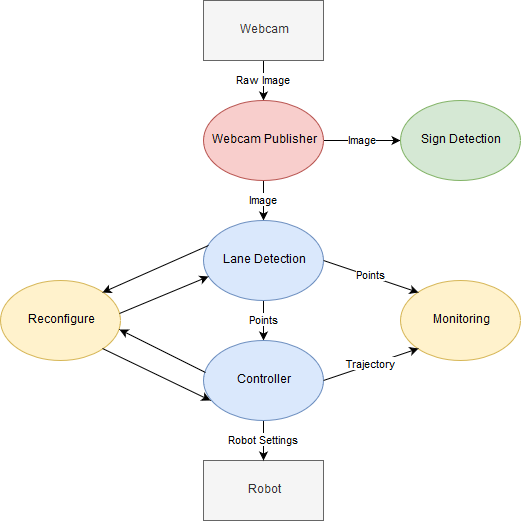
\includegraphics[width = 0.8\textwidth]{images/Projektaufbau.png}
	\caption{\"Ubersicht der einzelnen Komponenten des Projekts}
	\label{fig:projektaufbau}
\end{figure}
%TODO: der Controller heißt eigentlich trajectory_planning... Ist das bewusst so benannt? (Frederic)
\\
Abbildung \ref{fig:projektaufbau} zeigt die schematische Projektstruktur graphisch auf und erkl\"art sich folgenderma\ss{}en:
\begin{itemize}
\item Der \textbf{\textit{Webcam Publisher}} empf\"angt das rohe Kamerabild der \textbf{\textit{Webcam}} und nimmt Voreinstellungen, wie die Aufl\"osung vor. Dieses Bild wird an die Komponenten \textbf{\textit{Sign Detection}} und \textbf{\textit{Lane Detection}} verteilt.
\item Die \textbf{\textit{Lane Detection}} verarbeitet das Bild, ermittelt daraus Punkte der Fahrbahnmarkierungen und sendet diese dann an den \textbf{\textit{Controller}} weiter.
\item Mithilfe der Punkte wird durch den \textbf{\textit{Controller}} eine Trajektorie ermittelt und Motor- und Lenkeinstellungen berechnet, welche an das Roboterauto zur\"uckgegeben werden.
%TODO: Roboterauto richtiger Begriff? (Frederic)
\item Das \textbf{\textit{Monitoring}} nimmt die Ergebnisse der \textbf{\textit{Lane Detection}} und des \textbf{\textit{Controller}} und stellt diese graphisch zu \"Uberpr\"ufungszwecken dar.
\item \textbf{\textit{Reconfigure}} stellt dabei mehrere Werte sowohl der \textbf{\textit{Lane Detection}} als auch des \textbf{\textit{Controller}} w\"ahrend des Betriebs des Roboterautos, ein.
\end{itemize}
	\cleardoublepage
	\section{Bildverarbeitung}\label{sec:linien}

Als haupts\"achliche Quelle f\"ur die Erfassung und Verarbeitung der Umwelt des Fahrzeugs wurde das Bild
einer Webcam verwendet. Eine Kinect-Kamera mit Tiefenbild war zwar bereits auf dem Fahrzeug vorinstalliert,
jedoch beschlossen wir aus folgenden Gr\"unden, eine eigene Kamera zu verwenden:
\begin{itemize}
	\item Der flache Blickwinkel der Kinect erlaubte es nicht, den Boden unmittelbar vor dem Fahrzeug
	zu sehen. Die von uns verwendete Webcam dagegen konnte frei angebracht und der Blickwinkel
	(insbesondere dessen Steilheit) nach Belieben variiert werden.
	\item Die OpenCV-Bibliothek bot uns die M\"oglichkeit, den Webcam-Stream direkt einzulesen und
	daran Voreinstellungen vorzunehmen. Bei der Kinect w\"are hingegen eine Vorkonvertierung n\"otig
	geworden.
	\item F\"ur die von uns zu realisierenden Aufgaben (Fahrbahn- und Schildererkennung) war die
	zus\"atzliche Tiefenbild-Funktionalit\"at der Kinect wenig bis nicht relevant.
\end{itemize}

\begin{figure}[h]
	\centering
	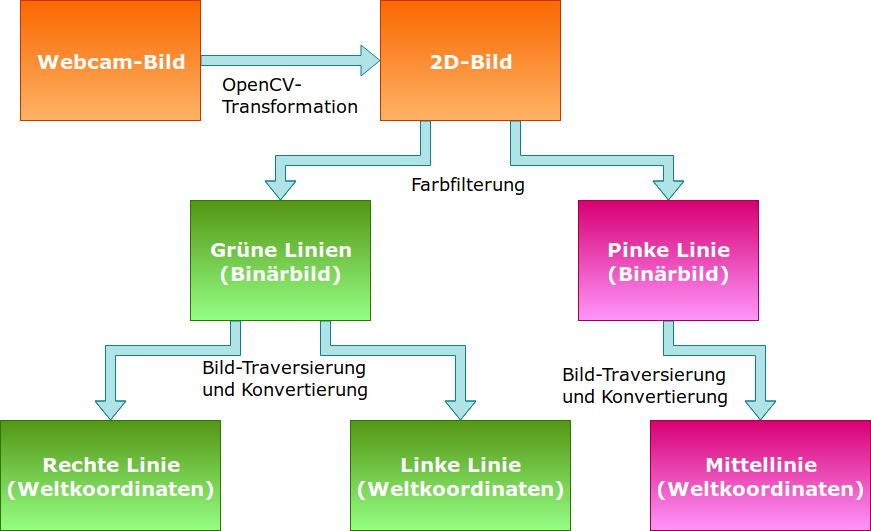
\includegraphics[width = 1.0\textwidth]{images/Bildverarbeitung.png}
	\caption{\"Ubersicht der einzelnen Schritte zur Bildverarbeitung}
	\label{fig:bildverarbeitung}
\end{figure}

Die groben Schritte, die im Rahmen der Bildverarbeitung durchgef\"uhrt werden, sind in
\figurename\ \ref{fig:bildverarbeitung} schematisch dargestellt.\\
Das eingelesene Webcam-Bild wird mithilfe der Bildverarbeitungs-Library OpenCV\cite{OCV} so transformiert, dass
der neue Bildausschnitt einer Draufsicht auf die Strecke aus der Vogelperspektive entspricht.
Davon ausgehend wird eine Farbfilterung vorgenommen, um die gr\"unen (Au\ss en-)Linien und die
pinke (innere) Linie jeweils in einem eigenen Bin\"arbild zu isolieren. Das Ergebnis wird
schlie\ss lich genutzt, um die Fahrzeugkoordinaten der einzelnen Linien zu bestimmen.\\
Die genauen Ma\ss nahmen, die f\"ur die Implementierung der einzelnen Verarbeitungsschritte getroffen 
wurden, werden im folgenden Abschnitt genauer vorgestellt.


\subsection{Kalibrierung der Kamera}
\label{subsec:kalibrierung}

Beim Anbringen der Webcam wurde ein Blickwinkel gew\"ahlt, der zum einen eine m\"oglichst gute Sicht auf die
Strecke unmittelbar vor dem Fahrzeug erm\"oglicht, aber gleichzeitig ausreichend viel Strecke nach
vorne erfasst (auch um Verkehrsschilder noch gut erkennen zu k\"onnen).\\
Um eine korrekte Transformation des aufgenommenen Bildes (im Folgenden auch als \textit{3D-Bild} bezeichnet)
in die Vogelperspektive (nachfolgend auch als \textit{2D-Bild} bezeichnet) erzielen zu
k\"onnen, wurde eine Kalibrierung f\"ur die eingestellte Kamera-Position vorgenommen.

Zu diesem Zweck wurde zun\"achst ein Referenz-Rechteck aus Papier angefertigt und dessen Ma\ss e
in Zentimetern ausgemessen.
F\"ur die Kalibrierung wurde dieses im zentralen Sichtfeld der Kamera platziert, zus\"atzlich wurde der
Abstand zum Fahrzeug bestimmt (siehe \figurename\ \ref{fig:testrechteck}).

\begin{figure}[h]
	\centering
	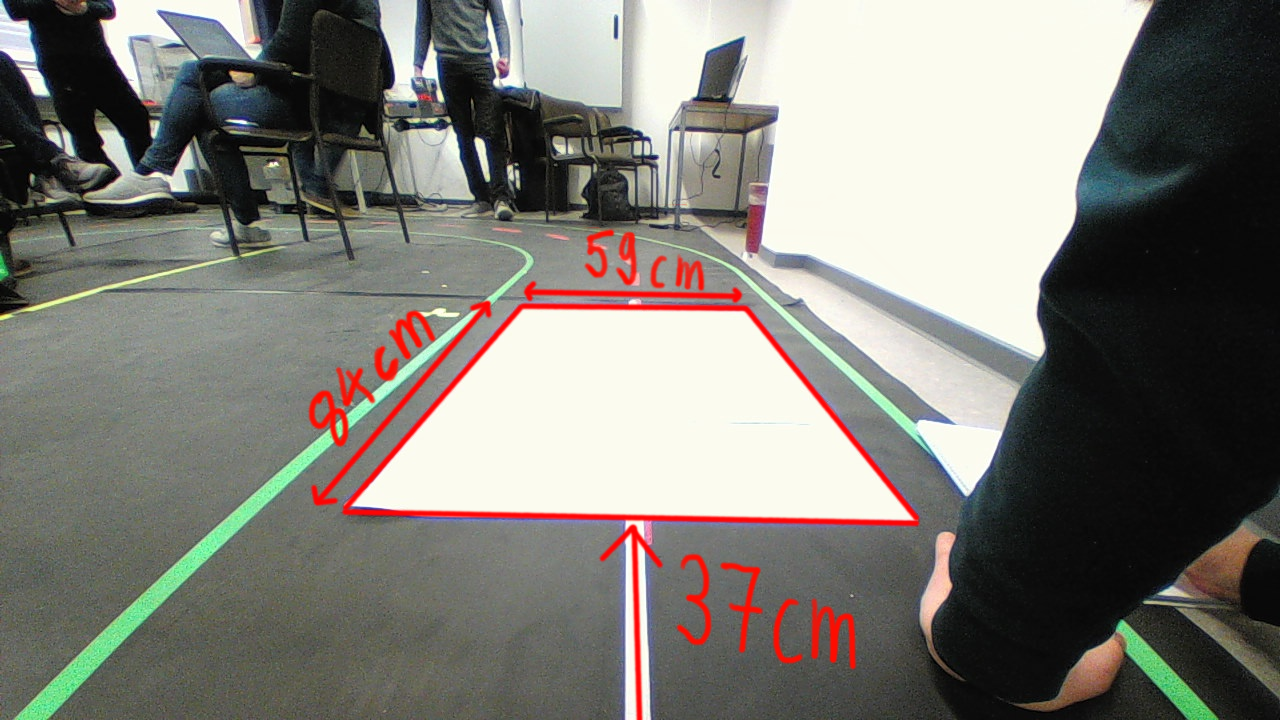
\includegraphics[width = 0.7\textwidth]{images/Testrechteck.png}
	\caption{Kalibrierung der Kamera mit dem Referenz-Rechteck}
	\label{fig:testrechteck}
\end{figure}

Anschlie\ss end wurden im aufgenommenen Bild die Pixelkoordinaten der Eckpunkte des Rechtecks ermittelt und notiert.

Zur Repr\"asentation einer festen Kamera-Kalibrierung und damit verkn\"upfter Informationen wurde eine eigene
C++-Klasse \texttt{CameraCalibration} geschrieben. Auf diese Weise l\"asst sich eine Kalibrierung leicht an mehreren
Stellen im Code verwenden. Instanzen der Klasse werden bei der Initialisierung einmalig
mit den ausgemessenen Pixelkoordinaten, den realen Ma\ss en des verwendeten Referenz-Rechtecks, dem gew\"unschten
Verh\"altnis von Pixeln zu Zentimetern im 2D-Bild sowie dem darzustellenden
Ausschnitt der Realit\"at in Zentimetern (in Blickrichtung und zu den beiden Seiten links
und rechts) initialisiert.\\
Davon ausgehend werden automatisch alle weiteren zur Erzeugung des Zielbildes n\"otigen Parameter berechnet.
Insbesondere wird \"uber die OpenCV-Funktion \texttt{getPerspectiveTransform} eine Transformationsmatrix
und deren Inverse abgespeichert, die jedem Pixel in der 3D-Perspektive eine Koordinate im 2D-Bild zuordnet
und umgekehrt.

\subsubsection{Umrechnung von Koordinaten}

Durch Anwendung der ermittelten Transformationsmatrix lassen sich einzelne Punkte des Webcam-Bilds zwar
in die Vogelperspektive mappen, jedoch war f\"ur die sp\"atere einfache Weiterverarbeitung von ermittelten Punkten
der Fahrbahnmarkierungen in der Fahrzeugregelung gew\"unscht, dass diese in Fahrzeugkoordinaten vorliegen.
Zu diesem Zweck musste eine Anpassung des Koordinatensytems sowie der verwendeten Einheiten vorgenommen
werden. Der Unterschied zwischen 2D-Bild-Koordinaten und den entsprechenden Koordinaten der realen
Welt ist in \figurename\ \ref{fig:koordinatensysteme} grafisch dargestellt.

\begin{figure}[h]
	\centering
	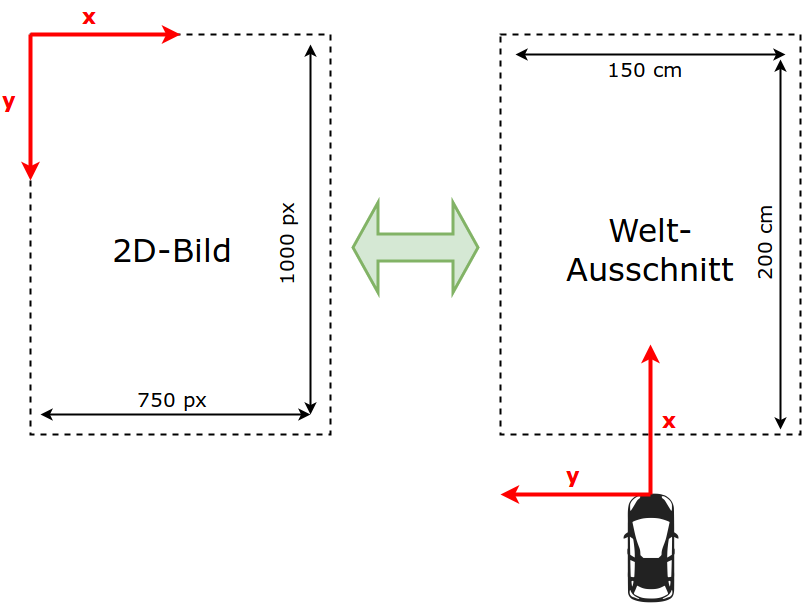
\includegraphics[width = 0.8\textwidth]{images/Koordinatenumrechnung.png}
	\caption{2D-Bild- vs. Fahrzeugkoordinaten}
	\label{fig:koordinatensysteme}
\end{figure}

Die ben\"otigte Funktionalit\"at zur Umrechnung zwischen 2D-Bild- und Welt-Koordinaten wird durch
Methoden in der Klasse \texttt{CameraCalibration} zur Verf\"ugung gestellt. Dabei werden die bei der Kalibrierung
abgespeicherten Informationen \"uber Gr\"o\ss e und Positionierung des Referenz-Rechtecks sowie der
Skalierungsfaktor f\"ur Pixel / Zentimeter verwendet
und das Koordinatensystem passend dazu neu bestimmt und ausgerichtet.\\

\textbf{TODO}\\
- Umrechnung der Koordinatensysteme ineinander, Formeln?\\

\subsection{Einlesen des Kamera-Bilds}

Zum Einlesen von Bildern der Webcam wurde ein Objekt vom OpenCV-Typ \texttt{VideoCapture} verwendet.
Dieses wurde in einer eigenen Klasse \texttt{CameraReader} gekapselt und um Zusatzfunktionalit\"at
erg\"anzt. So stellte sich heraus, dass zu jedem Auslesezeitpunkt f\"unf Webcam-Frames im Buffer des
Video-Streams gehalten werden, wovon das aktuellste das \"alteste ist. Um das neueste zu verwenden
und Lags zu vermeiden, verwirft der \texttt{CameraReader} daher die ersten vier Frames, sodass nur das letzte
tats\"achlich ausgelesen und im OpenCV-Bildformat (als \texttt{Mat}-Objekt) zur\"uckgegeben wird.

Zus\"atzlich wurde eine Methode zur Einstellung der Helligkeit, des Kontrasts, der S\"attigung und des
Farbtons des Kamera-Streams implementiert, um die Aufnahme bestm\"oglich auf aktuelle Lichtverh\"altnisse und zu
detektierende Farben anpassen zu k\"onnen.

Um eine modulare Softwarearchitektur zu gew\"ahrleisten, wurde die Funktionalit\"at zum Auslesen der Webcam
in eine eigene ROS-Node \texttt{webcam\_publisher} ausgelagert, welche den
\texttt{CameraReader} verwendet und ausgelesene Frames als ROS-Messages \"uber das ROS-Topic
\texttt{camera/frame} published.

\subsection{Weiterverarbeitung des Kamera-Bilds}

Das Herzst\"uck der eigentlichen Bildverarbeitung bildet die Klasse \texttt{ImageProcessor}. Sie kapselt
ein OpenCV-\texttt{Mat}-Objekt und enth\"alt verschiedene, zu gro\ss em Teil auf OpenCV basierende
Operationen, die darauf (in teilweise beliebiger
Reihenfolge) ausgef\"uhrt werden k\"onnen. Insbesondere stellt sie die Funktionalit\"at bereit, um

\begin{itemize}
	\item eine Transformation des Bildes in die Vogelperspektive anhand eines gegebenen
	\texttt{CameraCalibration}-Objekts vorzunehmen. Die Dimensionen des erzeugten Bilds bestimmen sich aus
	den in der Kalibrierung enthaltenen Informationen.
	\item eine Konvertierung des Bildes in den HSV-Farbraum vorzunehmen. Das aufgenommene Bild liegt
	zun\"achst in RGB vor, f\"ur die Bestimmung und Eingrenzung von Farb-Schwellwerten zur Linienerkennung
	ist HSV jedoch geeigneter: W\"ahrend (S)aturation und (V)alue angeben,
	wie \glqq wei\ss \grqq\ oder \glqq schwarz\grqq\ ein Pixel
	sein soll, l\"asst sich der Farbton durch den (H)ue-Kanal genau einstellen und auf einen engen
	Durchlassbereich begrenzen, was mit RGB nicht so leicht m\"oglich w\"are.
	\item eine Farbfilterung (nach einer vorherigen Transformation in den HSV-Farbraum) vorzunehmen. Dazu
	werden zwei Schwellwerte f\"ur die einzelnen Farbkan\"ale angegeben, die jeweils die untere bzw. die
	obere Schranke f\"ur den H-/S-/V-Wert darstellen. Das Ergebnis der Filterung ist ein Graustufen-Bild,
	in dem nur diejenigen Pixel wei\ss\ sind, deren Werte f\"ur \textit{alle} Kan\"ale zwischen den
	jeweiligen Schwellwerten liegen. Alle anderen Pixel sind dagegen schwarz (bzw. haben den Wert 0).
	Werden die Schwellwerte korrekt gew\"ahlt, lassen sich auf diese Weise gerade die rechte und linke
	Au\ss enlinie bzw. die Mittellinie der Fahrbahn in je einem Bin\"arbild isolieren.
	\item wei\ss e / nicht schwarze Punkte in einem (Bin\"ar-)Bild in einer bestimmten Pixel-Reihe
	von einer vorgegebenen Seite des Bildes aus zu suchen und die Pixel-Koordinaten zur\"uckzugeben.
	Diese Funktionalit\"at wird sp\"ater zur Ermittlung von Linienpunkten ben\"otigt.
\end{itemize} 

%TODO: nebeneinander dargestellt und kurz beschrieben: Quellbild - 2D-Bild - 2D-Bin\"arbild\\

\subsection{Detektion der Fahrbahnlinien}

F\"ur die Detektion der Fahrbahnlinien wurde eine abstrakte Oberklasse \texttt{LaneDetector} implementiert,
welche Methoden zur Ermittlung bzw. R\"uckgabe der einzelnen Linien deklariert und daf\"ur Objekte
weiterer Klassen verwendet. Die Idee hinter dieser
abstrakten Klasse war es, durch unterschiedliche Implementierungen Linienpunkte auf verschiedene Weise,
aber \"uber das gleiche Interface ermitteln zu k\"onnen.\\

\begin{figure}[h]
	\centering
	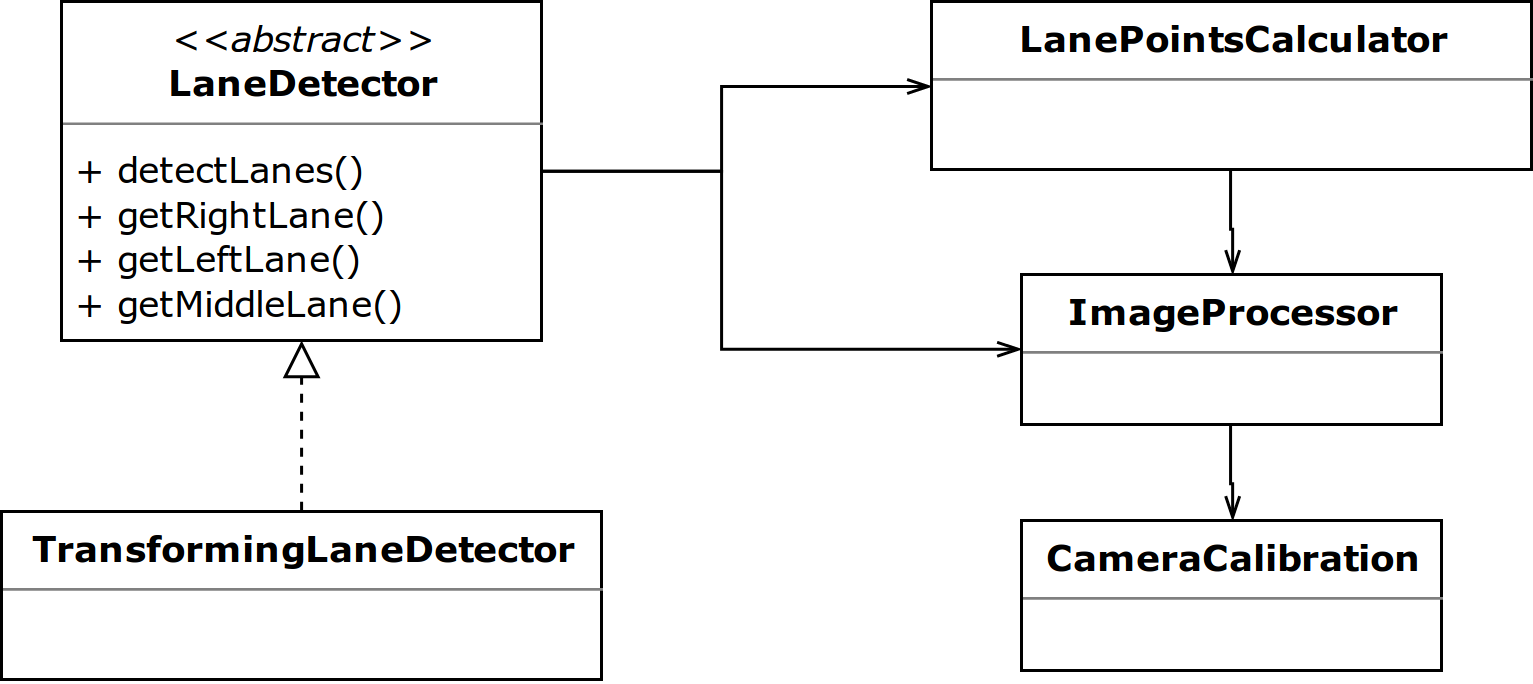
\includegraphics[width = 1.0\textwidth]{images/LaneDetectionKlassendiagramm.png}
	\caption{Vereinfachtes Klassendiagramm der Klassen zur Liniendetektion}
	\label{fig:lanedetection}
\end{figure}

Die f\"ur die Liniendetektion relevanten Klassen sind in \figurename\ \ref{fig:lanedetection} vereinfacht
dargestellt.

Die Singleton-Klasse \texttt{LanePointsCalculator} enth\"alt verschiedene Methoden, um mithilfe eines
\"ubergebenen \texttt{ImageProcessor}-Objekts Linien-Punkte im Bin\"arbild zu ermitteln. Bei der
Verwendung ist darauf zu achten, dass der \texttt{ImageProcessor} bereits ein fertig verarbeitetes
Graustufen-Bild enth\"alt.

Konkret implementiert wurden die Methoden aus \texttt{LaneDetector} in der Klasse
\texttt{TransformingLaneDetector}.\\
Diese verwendet zun\"achst den \texttt{ImageProcessor}, um das Quellbild in 2D zu transformieren und zwei
farbgefilterte Bilder (eines mit den gr\"unen und eines mit den pinken Linien) zu erhalten. Im n\"achsten
Schritt werden die Pixelkoordinaten der Linien mithilfe der Instanz des \texttt{LanePointsCalculator}
ermittelt und zwischengespeichert. Die endg\"ultigen Punkte der Linien in Pixelkoordinaten ergeben sich
erst aus einer Filterung der Zwischenergebnisse. Hier werden die Abst\"ande der gr\"unen Linien-Punkte
von der Mittellinie betrachtet, um sicherzustellen, dass es sich tats\"achlich um einen linken bzw.
rechten Punkt handelt (und nicht durch ein zwischenzeitlich schlechtes Bild Punkte der jeweils
gegen\"uberliegenden Linie falsch zugeordnet wurden). Nur Punkte, die rechts bzw. links von der
Mittellinie liegen, werden auch tats\"achlich als der entsprechenden Au\ss enlinie zugeh\"orig erkannt.

Schlie\ss lich wird das gespeicherte \texttt{CameraCalibration}-Objekt verwendet, um aus den Pixelkoordinaten
der jeweiligen Linie die entsprechenden Fahrzeugkoordinaten zu berechnen und zur\"uckzugeben.\\

F\"ur den Betrieb der Linienerkennung im Gesamtsystem existiert die ROS-Node \texttt{lane\_detection},
welche das ROS-Topic \texttt{camera/frame} subscribed und so die einzelnen Frames, die vom
\texttt{webcam\_publisher} ver\"offentlicht werden, empf\"angt. Zus\"atzlich werden die Farbschwellwerte
\"uber \texttt{rqt\_reconfigure}\cite{reconfigure} empfangen und gesetzt und zusammen mit
dem aktuellsten Frame an eine Instanz des \texttt{TransformingLaneDetector} \"ubergeben, welcher die
eigentlichen Berechnungen vornimmt.

Die ermittelten Punkte der einzelnen Fahrbahnlinien in Fahrzeugkoordinaten werden dann \"uber die Topics
\texttt{right\_lane}, \texttt{left\_lane} und \texttt{middle\_lane} gepublished, um von der
Trajektorienberechnung weiterverwendet werden zu k\"onnen. Au\ss erdem wird ein Bin\"arbild des fertig
verarbeiteten Webcam-Frames zu Monitoring-Zwecken ebenfalls gepublished.
	\cleardoublepage
	\section{Modellbildung und Regelung}
\label{sec:modelCtrl}
	
In Abschnitt \ref{sec:model} wird das Fahrzeug zun�chst mit Hilfe des Einspurmodells nach Ackermann \cite{ackermann} modelliert und anschlie�end die Geschwindigkeits- und Lenkwinkelbeziehungen zu den jeweiligen Stellgr��en bestimmt. In Abschnitt \ref{sec:traj} wird gezeigt, wie aus den erkannten Linien aus Kapitel \ref{sec:linien} eine Trajektorie bestimmt wird, welche als Referenzpfad oder zur direkten Steuerung genutzt werden kann. Im letzten Teil werden die zwei getesteten Regelkonzepte erl�utert und abschlie�end die genutzte Implementierung und eine kurze Beurteilung dar�ber gegeben.
\subsection{Modellierung}
In diesem Abschnitt wird zun�chst das Einspurmodell gezeigt und die daf�r n�tigen Abmessungen des Fahrzeugs genannt. Anschlie�end ist in den Abbildungen \ref{fig:lenkgroesse} der Verlauf der Lenkstellgr��e �ber den Lenkwinkel zu sehen und in Abb. \ref{fig:veloStell} der Verlauf der Geschwindigkeit bezogen auf die Geschwindigkeitstellgr��e.
\subsubsection{Ackermann Einspurmodell}\label{sec:model}
Das Fahrzeug wird zun�chst mit Hilfe des Einspurmodells nach Ackermann \cite{ackermann} modelliert. Das Einspurmodell ist eine �bliche Vereinfachung eines vollst�ndigen Modells eines Fahrzeugs mit 4 R�dern. Es fasst jeweils die Vorder- und Hinterr�der zu einem in der L�ngsachse liegendem Rad zusammen. F�r das Einspurmodell werden der Radstand und der Schwerpunkt des Fahrzeugs in der L�ngsachse ben�tigt. Der Radstand des Fahrzeugs betr�gt $L = 0.255 m$. Das Verh�ltniss zwischen Abstand Hinterachse zum Schwerpunkt zur Hinterachse betr�gt ca. $0.601$. Mit Hilfe des Einspurmodells kann f�r einen Lenkwinkel $\delta$ der sich daraus ergebende Kreisradius $R$ bei kontinuierlichem Lenkwinkel berechnet werden.
	
\begin{figure}[h]
\centering
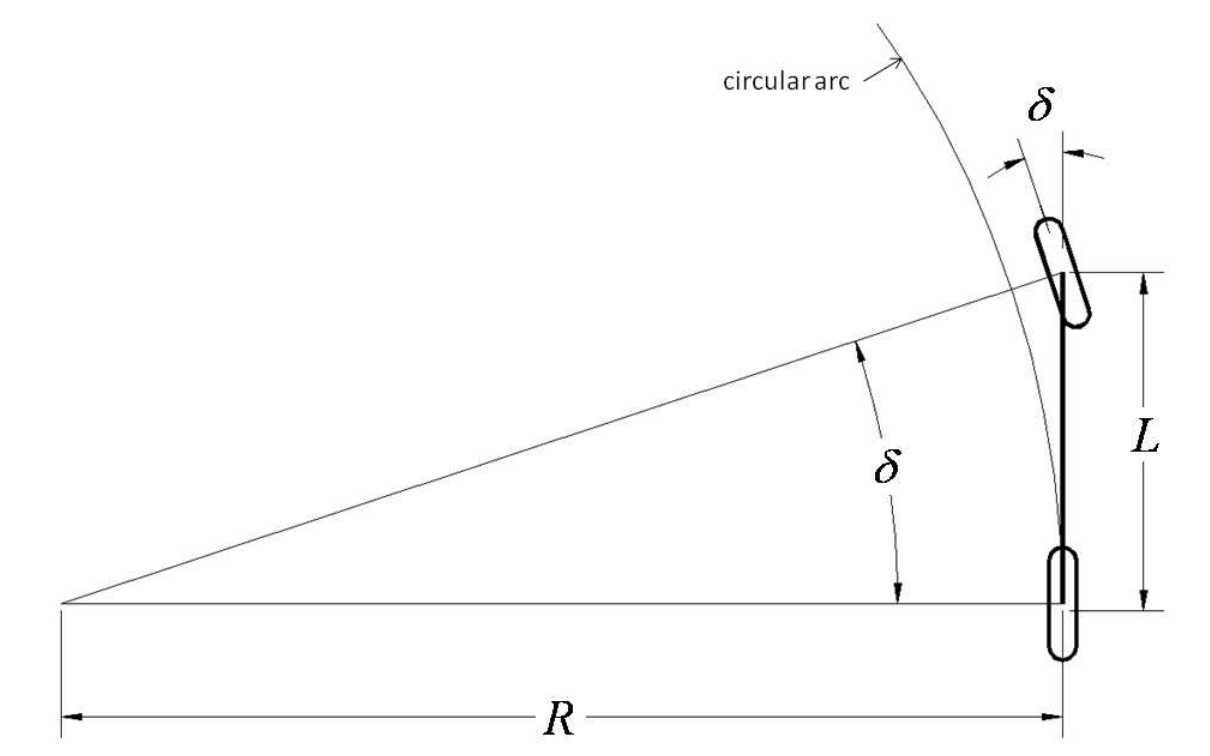
\includegraphics[width = 0.7\textwidth]{images/ackermann.png}
\caption{Ackermann Einspurmodell \cite{ackermann}}
\label{fig:ackermann}
\end{figure}
	
\subsubsection{Bestimmung der Lenkwinkel�bersetzung}\label{sec:lenk}
Im weiteren wird der Lenkwinkel f�r verschiedene Stellgr��en bestimmt. Dazu wurde f�r jeden Lenkwinkel wie folgt vorgegangen. Das Vorgehen hat sich im Projektseminar im vorausgehenden Jahr \cite{dontcode} bew�hrt.

\begin{itemize}
\item Das Fahrzeug wurde auf seinem Chassis aufgebockt und ein Rad �ber einem Winkelmesser zentriert.
\item Eine Geschwindigkeit von mindestens $300 \simeq 0.6\frac{m}{s}$ wurde eingestellt.
\item Die Lenkvorgabe wurde eingestellt und der Lenkwinkel abgelesen.
\end{itemize}

Aus den sich ergebenden Messpunkten wurde anschlie�end mit Hilfe von Matlab ein Polynom sechsten Grades (Gl.~\ref{eq:stell(lenkw)}) approximiert. Dabei ist zu beachten, dass die Koeffizieten $a_6$ und $a_5$ sehr klein sind:

\begin{align}
\begin{split}
\label{eq:stell(lenkw)}
U(\delta) =&5.726\cdot10^{-6}x^6-35.275\cdot10^{-6}x^5 -0.0044x^4\\ 
&+0.0126x^3+0.6745x^2-43.3355x+59.346
\end{split}
\end{align}
	
\begin{figure}[h]
\centering
% This file was created by matlab2tikz.
%
%The latest updates can be retrieved from
%  http://www.mathworks.com/matlabcentral/fileexchange/22022-matlab2tikz-matlab2tikz
%where you can also make suggestions and rate matlab2tikz.
%
\begin{tikzpicture}

\begin{axis}[%
width=4.521in,
height=2.7in,
at={(0.758in,0.481in)},
scale only axis,
xmin=-25,
xmax=25,
xlabel style={font=\color{white!15!black}},
xlabel={Lenkwinkel in Grad �},
ymin=-1000,
ymax=1050,
ylabel style={font=\color{white!15!black}},
ylabel={Lenkstellgroesse},
axis background/.style={fill=white},
axis x line*=bottom,
axis y line*=left,
xmajorgrids,
ymajorgrids,
legend style={legend cell align=left, align=left, draw=white!15!black}
]
\addplot [color=blue, draw=none, mark=*, mark options={solid, blue},mark size=1pt]
  table[row sep=crcr]{%
22	-1000\\
21	-925\\
19	-850\\
18	-775\\
17	-700\\
16	-625\\
15	-550\\
13	-475\\
11	-400\\
9.5	-325\\
8	-250\\
6	-175\\
4	-100\\
3	-50\\
2	-25\\
1	-10\\
0	70\\
-1	100\\
-2.5	175\\
-4	250\\
-6	325\\
-7.5	400\\
-9	475\\
-10.5	550\\
-13.5	625\\
-15.5	700\\
-17.5	775\\
-20	850\\
-20.5	925\\
-22	1000\\
};
\addlegendentry{Messung}

\addplot [color=green, solid, line width=1pt]
  table[row sep=crcr]{%
22	-995.475372508469\\
21	-944.206082620243\\
19	-824.782182082833\\
17	-699.435434651644\\
16	-638.662426049299\\
15	-580.434125640064\\
13	-473.309757857971\\
11	-378.83248310006\\
9.5	-314.975134330865\\
8	-255.370941700404\\
4	-103.534743889814\\
3	-64.6099058087682\\
2	-24.5971862536803\\
1	16.693191571643\\
0	59.3459841555404\\
-1	103.33897644747\\
-2.5	171.536302275685\\
-4	241.606891309475\\
-6	335.761337764135\\
-7.5	404.930495332449\\
-9	471.093087895453\\
-10.5	532.881256459638\\
-13.5	640.760148706949\\
-15.5	703.394004859994\\
-17.5	766.823844751602\\
-20	871.060107107013\\
-20.5	898.97885610975\\
-22	1006.28525865248\\
};
\addlegendentry{Modell}

\end{axis}
\end{tikzpicture}%
\caption{Lenkwinkel Stellgr��enbestimmung}
\label{fig:lenkgroesse} 
\end{figure}

Auff�llig ist, dass das Polynom nicht exakt durch $0$ verl�uft. Dies ist auch im folgenden Geschwindigkeitstest in Abschnitt \ref{sec:geschw} aufgefallen. Die Lenkstellgr��e musste auf $\simeq-70$ festgesetzt werden, um �ber eine l�ngere Strecke exakt geradeaus zu fahren. Dies kann allerdings auch daran gelegen haben, dass das linke vordere Rad geschliffen hat und das allradbetriebene Fahrzeug somit nach rechts gezogen hat. Der Antrieb des linken vorderen Rads ist sp�ter ganz ausgefallen.
	
Eine exaktere Methode w�re es, mit verschiedenen konstanten Geschwindigkeiten und Lenkwinkeln Kreise mit festen Radien abzufahren und mit Hilfe des Gyroskops und des Ackermann-Einspur-Modells die entsprechenden Lenkwinkel zu bestimmen. Dazu w�re eine Implementierung einer Odometrie n�tig, welche den zur�ckgelegten Weg und die entsprechende Pose aufzeichnet. Aufgrund der Komplexit�t und Zeitmangel wurde dies nicht zus�tzlich implementiert.
%TODO: kurz erkl�ren, warum das nicht gemacht wurde, z.B. einfach zus�tzlicher Implementierungsaufwand (Frederic)
%DONE


\subsubsection{Bestimmung der Geschwindigkeits�bersetzung}\label{sec:geschw}

Wie in Abschnitt \ref{sec:lenk} bereits genannt,
%TODO: zirkul�re Referenzierung nicht so gut - im vorigen Abschnitt wird Abschnitt 1.3 erw�hnt und hier wieder 1.2. Lieber chronologisch bleiben und nicht so viel vorgreifen (Frederic)
wurde ebenfalls eine Funktion bestimmt, die f�r die verschiedenen Stellgr��en die Geschwindigkeit in $\frac{m}{s}$ bestimmt. Dazu wurde die Zeit gemessen, die das Fahrzeug mit einer Stellgr��e ben�tigt, um eine bekannte Strecke zur�ckzulegen. Es wurde im Gegensatz zur Lenkwinkel�bersetzungsfunktion nicht ein sondern zwei Polynome bestimmt. Wie zu erkennen ist, gen�gt je ein Polynom ersten Grades f�r Vorw�rts- und R�ckw�rts-Fahren.

\begin{figure}[h]
\centering
% This file was created by matlab2tikz.
%
%The latest updates can be retrieved from
%  http://www.mathworks.com/matlabcentral/fileexchange/22022-matlab2tikz-matlab2tikz
%where you can also make suggestions and rate matlab2tikz.
%
\begin{tikzpicture}

\begin{axis}[%
width=4.521in,
height=3.0in,
at={(0.758in,0.481in)},
scale only axis,
xmin=-600,
xmax=800,
xlabel style={font=\color{white!15!black}},
xlabel={Stellgroesse Uv der Geschwindigkeit},
ymin=-1.5,
ymax=2,
ylabel style={font=\color{white!15!black}},
ylabel={Geschwindigkeit in m/s},
axis background/.style={fill=white},
axis x line*=bottom,
axis y line*=left,
xmajorgrids,
ymajorgrids,
legend style={legend cell align=left, align=left, draw=white!15!black, at={(axis cs:-550,1.8)},anchor=north west}
]

\addplot [color=blue, draw=none, mark=*, mark options={solid, blue}, mark size = 1pt]
  table[row sep=crcr]{%
-500	-0.949999999999989\\
-400	-0.819999999999993\\
-300	-0.600000000000023\\
-200	-0.240000000000009\\
-170	-0.099999999999994\\
170	0.100000000000002\\
200	0.259999999999991\\
300	0.600000000000023\\
400	0.833300000000008\\
500	1\\
700	1.58000000000004\\
};
\addlegendentry{Messung}

\addplot [color=green, solid, line width= 1pt]
  table[row sep=crcr]{%
-500	-1.005\\
-200	-0.300000000000011\\
-170	-0.1\\
};
\addplot [color=green, solid, line width= 1pt, forget plot]
  table[row sep=crcr]{%
170 0.1	\\
200	0.294947297297313\\
700	1.56702162162162\\
};
\addlegendentry{Modell}

\draw [dashed] (-170,-1.5) -- (-170,2);
\draw [dashed] (170,-1.5) -- (170,2);

\end{axis}
\end{tikzpicture}%
\caption{Geschwindigkeit Stellgr��enbestimmung}
\label{fig:veloStell} 
\end{figure}

Der Verlauf ist ebenso wie die Lenkwinkel�bersetzung nicht exakt, da mit der Hand gestoppt wurde und nicht vollkommen klar ist, ob das Fahrzeug trotz Vorlauf schon die exakte Geschwindigkeit erreicht hat. D.h. das Fahrzeug ist nicht direkt an der Startlinie der abgemessenen Strecke losgefahren, sondern davor um sicherzustellen, dass die Zielgeschwindigkeit erreicht ist.
%TODO: verstehe ich nicht ganz - was ist "Vorlauf", warum ist das nicht klar? (Frederic)
%DONE
Eine exaktere Methode h�tte wiederum eine Odometrie verlangt oder dass die 'Wheelticks' (Gl.~\ref{eq:vel}) der Hallsonde �ber einen Zeitraum gemessen worden w�ren. 'Wheelticks' sind die mit Hilfe einer Hallsonde gemessenen Umdrehungen eines Rades. Eine Hallsonde misst Magnetfelder und kann Metalle sensieren. Dies wird dazu genutzt, in dem ein sensiertes Metall im Rad bei jeder Umdrehung dieses erkannt wird.
%TODO: du setzt hier voraus, dass der Leser wei�, was 'Wheelticks' genau sind und von welcher Hallsonde gesprochen wird - ich zumindest wei� nicht, was gemeint ist. :D (Frederic)
%DONE?
\begin{align}\label{eq:vel}
v = \frac{num_{wheelticks }\cdot2\pi r_{wheel}}{t}
\end{align}
%TODO: w�rde die Formel vll. eher weglassen, sehe keinen Mehrwert darin, die noch mit aufzuf�hren (Frederic)


\subsection{Trajektorienberechnung}\label{sec:traj}

In diesem Abschnitt wird beschrieben, wie aus den erkannten Fahrbahnmarkierungen aus Kapitel \ref{sec:linien} eine Referenztrajektorie geplant wird. Ben�tigt wird mindestens eine Punkteschar im Fahrzeug- bzw. Weltkoordinatensystem einer Fahrbahnmarkierung. Aus dieser kann mit Hilfe einer Verschiebung der Punkte eine Trajektorie berechnet werden. Sind Linien mehrerer Markierungen vorhanden, ist es au�erdem m�glich, eine Mittelung vorzunehmen.

\begin{figure}[h]
\centering
%\documentclass[tikz]{standalone}
%\usepackage[T1]{fontenc}
%\usepackage[utf8]{inputenc}
%\usepackage{pgfplots}
%\usepackage{grffile}
%\pgfplotsset{compat=newest}
%\usetikzlibrary{plotmarks}
%\usetikzlibrary{arrows.meta}
%\usepgfplotslibrary{patchplots}
%\usepackage{amsmath}
%
%\begin{document}
\begin{tikzpicture}

\begin{axis}[%
width=4.521in,
height=3.0in,
at={(0.758in,0.481in)},
scale only axis,
xmin=-50,
xmax=50,
xlabel style={font=\color{white!15!black}},
xlabel={lateraler Abstand [cm]},
ymin = 0,
ymax=150,
ylabel style={font=\color{white!15!black}},
ylabel={longitudinaler Abstand [cm]},
axis background/.style={fill=white},
axis x line*=bottom,
axis y line*=left
,
xmajorgrids,
ymajorgrids,
]

\draw[color=green] (-25,0) to[out=90,in=305-70] (-10,150);
\draw[color=green] (25,0) to[out=90,in=305-70] (40,150);
\draw[red, dashed] (0,0) to[out=90,in=305-70] (15,150);
\draw[color=blue] (12.5,0) to[out=90,in=305-70] (27.5,150);
\draw[color=green] (-15,135) node[left] {$Linker Rand$};
\draw[color=red] (10,135) node[left] {$Mittellinie$};
\draw[color=green] (24.5,30) node[right] {$Rechter Rand$};
\draw[color=blue] (18,110) node[right] {$Trajektorie$};



\end{axis}
\end{tikzpicture}%
%\end{document}

\caption{Trajektorienbestimmung}
\label{fig:veloStell} 
\end{figure}

Um die Trajektorie zu bestimmen wurden die verf�gbaren R�nder der Fahrbahn mit Hilfe der Numerik-Library alglib \cite{alglib} interpoliert. Die $i$ Punkte der erkannten Linien werden als St�tzstellen zur Trajektorienberechnung genutzt. Zun�chst wird eine Linie in Abh�ngigkeit der Bogenl�nge $s$ (Gl.~\ref{eq:s}) parametrisiert. Dazu wird zu jeder
%TODO: hier w�re noch eine kurze Erkl�rung der St�tzstelle i gut. au�erdem finde ich die Beschreibung "linear akkumuliert" zu kompliziert / umst�ndlich (Frederic)
St�tzstelle $i$ der linear aufsummierte Weg $s_i$ zwischen den St�tzstellen berechnet:

\begin{align}\label{eq:s}
s_i = \sum\limits_{i=1}^{n} \sqrt{(x_i-x_{i-1})^2+(y_i-y_{i-1})^2} \text{ mit: } s_0 = 0
\end{align}

Daraufhin werden die Linien durch zwei kubische Splines $x(s)$ und $y(s)$ interpoliert. Abh�ngig von der Bogenl�nge $s$, oder dem auf dem Spline zur�ckgelegten Weg, k�nnen mit diesen beiden Splines auch zwischen den St�tzstellen Punkte der Linien bestimmt werden.
%TODO: das "somit" erschlie�t sich mir nicht - worauf bezieht sich das? Die M�glichkeit der Interpolation von Rundkursen ist m.M. nach noch keine logische Konsequenz daraus, zwei Splines zu haben - oder m�sste noch genauer erkl�rt werden. (Frederic)
%REVIEW
Die Parametrisierung erlaubt es zum Beispiel geschlossene Rundkurse durch zwei solcher Splines zu interpolieren, da diese Polynome jeweils eindeutig sind. Die Splines sind eine Schar von Polynomen (Gl.~\ref{eq:xs}~und~\ref{eq:ys}), dritten Grades im Fall von kubischen Splines, welche ihre G�ltigkeit im Bereich zwischen den St�tzstellen $i$ und $i+1$ haben. Die Splines sind �berall, au�er in der ersten und letzten St�tzstelle, zweifach stetig differenzierbar.

\begin{align}
\begin{split} \label{eq:xs}
x(s) = a_i s^3+b_i s^2+c_i s+d_i
\end{split}\\
\begin{split} \label{eq:ys}
y(s) = a_i s^3+b_i s^2+c_i s+d_i
\end{split}
\end{align}

%Es ist notwendig die Punkteschar zu parametrisieren, um die Eindeutigkeit  zu gew�hrleisten.
%TODO: die Eindeutigkeit wovon? (Frederic)
%DONE verschoben nach oben, um damit auch den anderen TODO zu l�sen
%REVIEW
Die Splines erlauben es, in jedem Punkt die Steigung (Gl.~\ref{eq:steigung}) und Kr�mmung (Gl.~\ref{eq:curv}) der Kurve zu berechnen.
\begin{align}
\label{eq:steigung}
\dot{f}(x,y) = atan2\left(\frac{\dot{y}}{\dot{x}}\right)
\end{align}
\begin{align}
\label{eq:curv}
\kappa = \frac{\ddot{x}\dot{y}-\ddot{y}\dot{x}}{\sqrt[3]{\dot{x}^2+\dot{y}^2}}
\end{align}

%TODO: ALLGEMEIN: du gehst hier bei den ganzen Formeln davon aus, dass der Leser schon sehr tief in der Materie drin ist und genau wei�, welche Variablen was bedeuten und was da jeweils konkret berechnet wird - ist aber nicht unbedingt der Fall. Finde, man wird ganz sch�n mit Formeln bombardiert, ohne dass diese genauer erkl�rt werden. Ich w�rde alle verwendeten Parameter (s, x, y, ...) auch erst mal einf�hren. Oder im Zweifel auf die ein oder andere Formel verzichten. (Frederic)

\subsection{Regelung}\label{sec:ctrl}
In diesem Kapitel werden zwei verschiedene Regelkonzepte aufbauend auf die Referenztrajektorie aus Abschnitt~\ref{sec:traj} gezeigt, die im Laufe des Projektseminars implementiert und getestet wurden. Zun�chst wird gezeigt, wie mit Hilfe eines PID-Reglers ein Fehler ausgeregelt wird. Einerseits kann dieser aufgrund der vorliegenden Modellierung der Lenkwinkel�bersetzung aus Abschnitt \ref{sec:lenk} 
%TODO: "ebenfalls": was ist das andere, worauf hier Bezug genommen wird? (Frederic)
den aktuellen Lenkwinkel korrigieren. Dazu muss die Ausgabe des Reglers lediglich dem Polynom (Gl.~\ref{eq:stell(lenkw)}) �bergeben werden. Andererseits kann der laterale Fehler in $cm$ genutzt werden, um das Stellsignal direkt zu steuern. Weiterhin wird im zweiten Abschnitt dieses Teils eine Regelung gezeigt, die aus der Kr�mmung (Gl.~\ref{eq:curv}) der Trajektorie direkt den n�tigen Lenkwinkel des Fahrzeugs berechnet, um die Trajektorie abzufahren. Dazu wird das Ackermann-Einspur-Modell aus Abschnitt \ref{sec:model} benutzt.
	
\subsubsection{PID-Regler}\label{sec:pid}

Der PID-Regler in (Abb.~\ref{fig:PID-System}) erh�lt den aktuellen lateralen Fehler, zwischen longitudinaler Achse und der Referenztrajektorie, in einem bestimmten Abstand zum Fahrzeug als auszuregelnden Fehler.
%TODO: da stimmt was nicht mit der Satzstellung - ist kein richtiger Satz :D (Frederic)
%DONE Facepalm
Der Regler besteht aus drei verschiedenen Elementen:


\begin{itemize}
	\item Das P-Glied verst�rkt den aktuellen Fehler linear.
	\item Das I-Glied summiert den Fehler �ber die Zeit auf und hat somit ein \glqq Ged�chtnis\grqq . I-Glieder eignen sich besonders, um bleibende Regelabweichungen zu verhindern.
	\item Weiterhin wurde ein kleiner D-Anteil benutzt, um schnell auf auftretende Fehler reagieren zu k�nnen. D-Glieder verst�rken die �nderung des Fehlers.
\end{itemize}


\begin{figure}[h]
\centering
%\documentclass{article}
%
%\usepackage{tikz}
%\usetikzlibrary{shapes,arrows}
%\begin{document}

\tikzstyle{block} = [draw, fill=white, rectangle, 
    minimum height=3em, minimum width=6em]
\tikzstyle{sum} = [draw, fill=white, circle, node distance=1cm]
\tikzstyle{input} = [coordinate]
\tikzstyle{output} = [coordinate]
\tikzstyle{pinstyle} = [pin edge={to-,thin,black}]

\begin{tikzpicture}[auto, node distance=2cm,>=latex']

    \node [input, name=input] {};
    \node [sum, right of=input] (sum) {};
    \node [block, right of=sum] (controller) {PID-Regler};
    \node [block, right of=controller, pin={[pinstyle]above:D},
            node distance=3cm] (system) {Fahrzeug};

    \draw [->] (controller) -- node[name=u] {$u$} (system);
    \node [output, right of=system] (output) {};
    \node [block, below of=u] (measurements) {Bildverarbeitung};

    \draw [draw,->] (input) -- node {$r$} (sum);
    \draw [->] (sum) -- node {$e$} (controller);
    \draw [->] (system) -- node [name=y] {$y$}(output);
    \draw [->] (y) |- (measurements);
    \draw [->] (measurements) -| node[pos=0.99] {$-$} 
        node [near end] {$y_m$} (sum);
\end{tikzpicture}
%\end{document}
\caption{PID-Regler mit System}
\label{fig:PID-System} 
\end{figure}

Im Speziellen wurde der PID-Regler bezogen zur Standardmodellierung so angepasst, dass falls der Fehler am Sinken ist, der integrierende Anteil schneller abgebaut wird.  
%TODO: schneller als was? was hei�t "abgebaut"? (Frederic)
Beim Standardmodell eines PID-Reglers steigt der I-Anteil weiterhin an, selbst wenn der Fehler bereits ausgeregelt wird. Der exakte Entwurf des implementierten PID-Reglers ist in Abbildung \ref{fig:PID} zu sehen. F�r den Standardentwurf w�rde der Fehler \textit{err} aus Abbilung~\ref{fig:PID}, wie beim P und D-Glied in den Integrator und von dort in den Verst�ker einflie�en.  
%TODO: kurze Beschreibung, was f�r eine Art von Entwurf / Skizze das ist (Frederic)



\begin{figure}[h]
\centering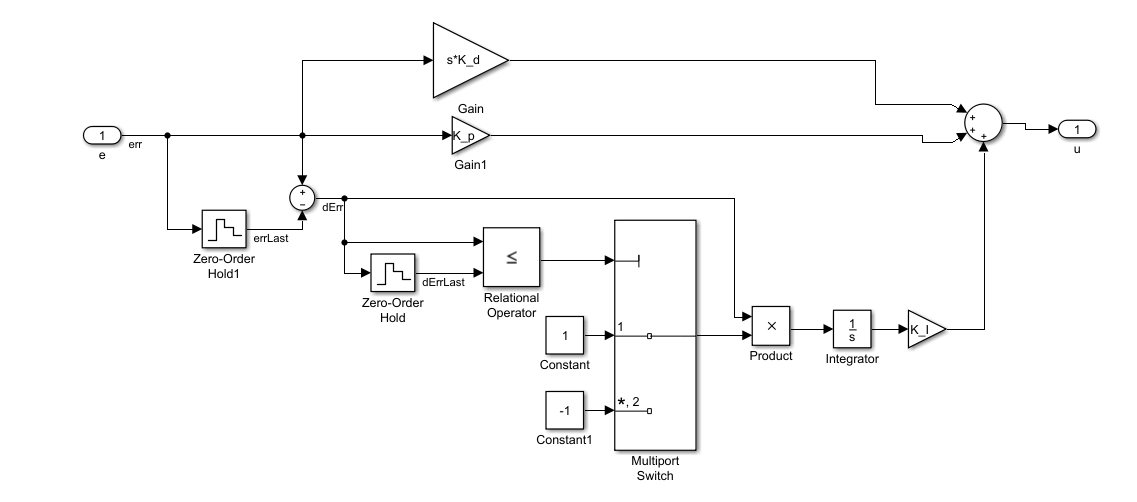
\includegraphics[width=\textwidth]{images/PID_modell.PNG} 
\caption{PID-Regler}
\label{fig:PID} 
\end{figure}


\subsubsection{Lenkwinkelbestimmung durch die Trajektorie}\label{sec:curv2lenk}

Die direkte Bestimmung des Lenkwinkels mit Hilfe einer Referenztrajektorie \cite{ackermann} ist eher eine Art der Steuerung als eine Regelung. Diese Methode ben�tigt eine Trajektorie, wie sie in Abschnitt \ref{sec:traj} beschrieben wird. Weiterhin wird ein m�glichst exaktes Fahrzeugmodell (siehe Abschnitt \ref{sec:model}) ben�tigt. Nun wird ein Punkt auf der Trajektorie gew�hlt, der sich eignet, darauf zu regeln. An diesem Punkt wird die Kr�mmung wie in Gleichung \ref{eq:curv} bestimmt. Aus dem Einspurmodell nach Ackermann ergibt sich, dass f�r eine Kurvenfahrt konstanten Radius der laterale Abstand ($R$ siehe Abb.~\ref{fig:ackermann}) zwischen Hinterachse des Fahrzeugs und dem augenblicklichen Kr�mmungszentrum (engl. ICC) dem Kehrwert der Kr�mmung $\kappa$ entspricht. 

\begin{align}
R = \frac{1}{\kappa}
\end{align}

Aus diesem Zusammenhang l�sst sich nun direkt mit Hilfe der Kr�mmung der Trajektorie der ben�tigte Lenkwinkel berechnen:

\begin{align}\label{eq:lenkwinkel_complex}
\delta = \arctan\left(\frac{L_{rear,front}}{\sqrt{\frac{1}{\kappa^2}-L_{rear,CoG}^2}}\right)
\end{align}

%TODO: auch hier wieder: Erkl�rung der Symbole in der Formel (Frederic)
\begin{itemize}
\item $L_{rear,front}$ entspricht dem Radstand des Fahrzeugs.
\item $L_{rear,CoG}$ entspricht dem Abstand zwischen Hinterachse und dem Schwerpunkt (engl. center of gravity) des Fahrzeugs.
\end{itemize}
Im Fall von sehr gro�en Kurvenradien ($\frac{1}{\kappa}=R >> L_{rear,CoG}$) im Vergleich zur Fahrzeugl�nge ist allerdings auch eine Vereinfachung der Gleichung \ref{eq:lenkwinkel_complex} m�glich \cite{acker}:

\begin{align}
\delta = \arctan \frac{L}{R} = \arctan L \cdot \kappa
\end{align}

\subsection{Implementierung}\label{sec:ctrlImpl}

Der PID-Regler wurde als Klasse \textit{Controller} implementiert und ist in der Lage verschiedene Inputs auszuregeln. Dabei ist es m�glich nach dem genannten Konzept einen einzelnen Fehler an einem Punkt auf der Trajektorie oder Schaar von Fehlern zu �bergeben. Zur Berechnung der Trajektorie wurde eine weitere Klasse, die auf die \textit{alglib} \cite{alglib} aufbaut implementiert. Diese ben�tigt lediglich zwei Vektoren mit den Punkten einer Linie als Input. Die Punkte werden daraufhin interpoliert und zwei kubische Splines (siehe. Gl.~\ref{eq:xs}~\&~\ref{eq:ys}) werden bestimmt. Es ist m�glich verschiedene Operationen der \textit{alglib} auf den Spline-Objekten der Klasse anzuwenden oder aus einer oder zwei solcher Instanzen der Klasse, die eine Linie interpolieren eine Trajektorie zu bestimmen. Dazu kann man einen Offset in lateraler Richtung zur Linie addieren lassen oder zwei Linien gewichtet Vermischen. Die \textit{alglib} selbst bietet Funktionen an die Ableitungen eines Splines an einem Punkt zu bestimmen. Diese wurde im Vorlauf hinreichend an Beispielen getestet, um mit Hilfe der Ableitungen die Kr�mmung zu bestimmen. Dies war n�tig, um die Machbarkeit des zweiten Regelentwurfs (siehe~\ref{sec:curv2lenk}) theoretisch nachzuweisen. Dazu wurden Kreise und festdefinierte stetige Kurven interpoliert und anschlie�end die bekannte Kr�mmung durch die Funktionen der \textit{alglib} �berpr�ft. In der Praxis waren die Splines der \textit{alglib} jedoch nicht nutzbar, da es regelm��ig auf Geradenst�cken in manchen Punkten zu extrem gro�en Kr�mmungen (kleinen Kurvenradien) gekommen ist. Deshalb wurde eine weitere Klasse \cite{poly} getestet, welche mit Hilfe eines Least-Squares-Verfahrens ein Polynom bestimmt, dass die Punkteschaar interpoliert. Die darauf bestimmten Ableitungen haben robustere Ergebnisse geliefert, jedoch kam es trotzdme noch zu gr��eren Regelabweichungen. Weshalb letztlich der PID-Regler zum Einsatz kam, welcher robustere Fahrergebnisse geliefert hat. \\
Au�erdem wurde noch eine Vehicle Klasse implementiert, der das Fahrzeugmodell zugrunde liegt. Diese erm�glicht es zum Beispiel aus dem berechneten Lenkwinkel der Trajektorie eine Lenkstellgr��e zu bestimmen.

%TODO: was noch fehlt in dem Kapitel ist eine Aussage, welchen Ansatz wir letztendlich konkret verwendet haben (und evtl. warum) (Frederic)
%TODO: ich w�rde auch noch, zumindest kurz, konkret auf die Implementierung eingehen (z.B. es wurde die Klasse daf�r geschrieben und die Node daf�r verwendet). Im Moment bleibt es noch sehr abstrakt und es wird mehr erkl�rt, mit welchen Formeln man welches Problem l�sen K�NNTE. (Frederic)
	\cleardoublepage
	\section{Monitoring und Debugging}
\label{sec:monitoring}

%TODO:\\
%- image\_publisher\\
%- image\_viewer\\
%- draw\_grid\_on\_camera\\
%- rqt\_reconfigure: (Kamera-Setup, Farbwerte, Trajektorienparameter)\\

In diesem Kapitel werden die verschiedenen Mechanismen vorgestellt, welche von uns f\"ur Monitoring und Debugging eingesetzt wurden. Ein Teil davon war hilfreich bei der Entwicklung einzelner Funktionalit\"aten, ein anderer hat die Fehlersuche im Betrieb wesentlich vereinfacht.

\subsection{image\_publisher und image\_viewer}
Mit ROS hat man die M\"oglichkeit, einzelne Nodes sehr einfach auszutauschen und somit die Funktionalit\"at schnell anzupassen, solange die Schnittstelle (die Messages) gleich bleiben. Dies haben wir uns f\"ur eine fr\"uhe Phase der Entwicklung zu Nutze gemacht. Im laufenden Betrieb liest die Bildverarbeitung Bilder aus der Webcam und ver\"offentlicht sie auf dem Topic \texttt{camera/frame}. Hierf\"ur werden aber das Fahrzeug und die dort installierte Webcam ben\"otigt.

Um auch lokal am Laptop testen zu k\"onnen, haben wir eine ROS-Node \texttt{image\_publisher} geschrieben, welche zuvor aufgenommene und lokal abgespeicherte Bilder \"offnet und published. Somit sind wir in der Lage unabh\"angig vom Fahrzeug die Bildverarbeitung zu testen und ggf. Parameter anzupassen.\\

Der umgekehrte Fall ist die Anzeige der Bilder. Im laufendem Betrieb sollten die Aufnahmen der Webcam angezeigt werden k\"onnen. Dazu wird in der ROS-Node \texttt{image\_viewer} das Topic \texttt{camera/frame} ausgelesen und das darin befindliche Bild angezeigt.
Zus\"atzlich werden die erkannten Punkte der Fahrbahnlinien sowie die daraus erzeugte 
Trajektorie aus den entprechenden Topics ausgelesen, \"uber ein 
\texttt{CameraCalibration}-Objekt zur\"uck in Bildkoordinaten transformiert und in
das angezeigte Bild eingezeichnet, wodurch eine Kontrolle der aktuell ermittelten
Linien in Echtzeit m\"oglich ist (siehe Abbildung \ref{fig:monitoring}).

\begin{figure}[!htb]
	\centering
	\begin{minipage}{.5\textwidth}
		\centering
		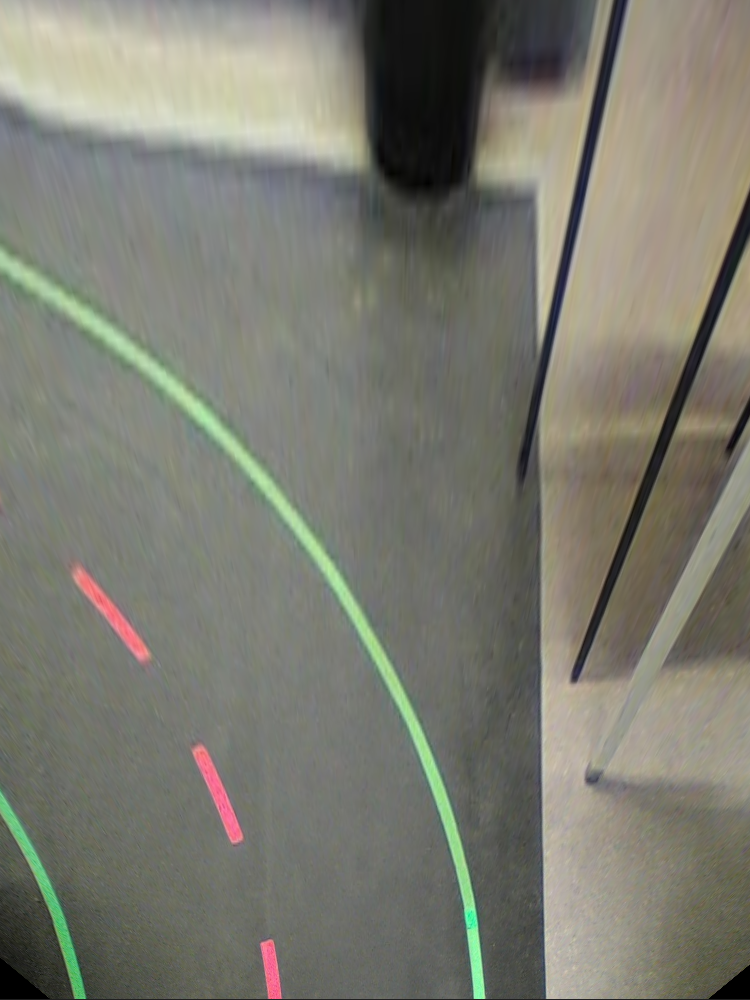
\includegraphics[width=0.7\linewidth]{images/transformed_color}
	\end{minipage}%
	\begin{minipage}{0.5\textwidth}
		\centering
		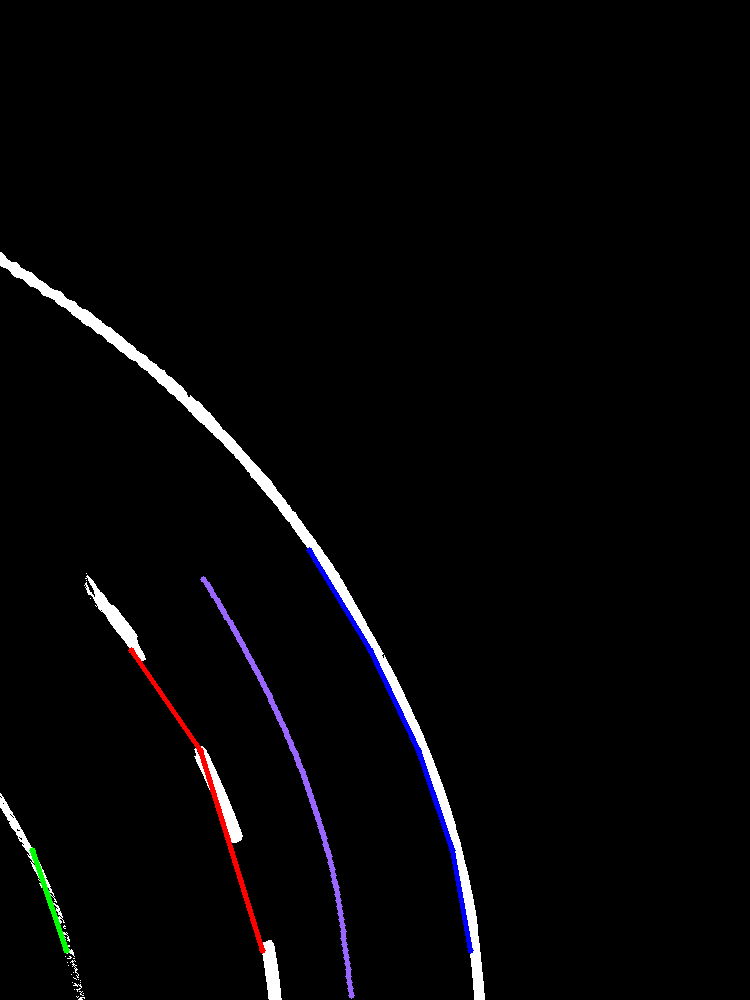
\includegraphics[width=0.7\linewidth]{images/trajectory}
	\end{minipage}
\label{fig:monitoring}
\caption{2D-Bild und zugeh\"origes Monitoring-Bild des \texttt{image\_viewer}}
\end{figure}

\subsection{Einzeichnen eines Rasters ins Bild und Aufnehmen von Fotos}
F\"ur die Transformation der Kamera-(3D-)Pixelkoordinaten in die Vogelperspektive (2D) ist wie in Abschnitt \ref{subsec:kalibrierung} beschrieben eine Kalibrierung der Kamera notwendig.
Um das hierf\"ur verwendete Referenz-Rechteck zentral im Sichtfeld der Kamera
platzieren zu k\"onnen, ist ein im Bild der Kamera eingezeichnetes Raster hilfreich.
Mangels geeigneter Webcam-Tools entschieden wir uns, eine eigene Hilfs-Node
zu implementieren, die das aktuelle Frame auf dem Topic
\texttt{camera/frame} mit Hilfe von OpenCV
zusammen mit einem Grid-Overlay anzeigt.

Sp\"ater wurde zus\"atzlich eine Funktion implementiert, um zu jeder Zeit per
Tastendruck ein Foto abspeichern zu k\"onnen, was sich zum Erstellen von Test-Bildern,
aber auch von Trainingss\"atzen f\"ur die Schildererkennung bezahlt machte.

\subsection{rqt\_reconfigure}
Da unsere Software auf dem Fahrzeug eine Viehlzahl an einzustellenden Parametern aufweist, haben wir uns f\"ur eine M\"oglichkeit zur dynamischen Rekonfiguration zur Laufzeit entschieden. Die ROS-Bibliothek bietet hier mit \textit{rqt\_reconfigure}\cite{reconfigure} einen entsprechenden Dienst an. Nachdem die zu \"andernden Parameter in einer Konfigurations-Datei vorkonfiguriert worden sind, muss man in den entsprechenden Nodes noch eine Callback Methode implementieren, welche die ge\"anderten Parameter \"ubernimmt. Somit ist man in der Lage, im laufenden Betrieb bestimmte Parameter zu ver\"andern.

Wir haben rqt\_reconfigure konkret f\"ur das Setup der Kamera (Parameter wie Helligkeit, Kontrast, ...), die Einstellung der Farbschwellwerte f\"ur die Linienerkennung (gr\"une und pinke Linie) sowie f\"ur Reglereinstellungen in der Trajektorienplanung verwendet.

\subsection{Netzwerkkommunikation}
Um die umfangreichen Optionen von Monitoring und Rekonfiguration sinnvoll nutzen zu k\"onnen, bedurfte es einer Kommunikation \"uber das Netzwerk. Da hier keine Zeitkritischen Funktionen ausgef\"uhrt werden, l\"auft die Kommunikation in unserem Projekt \"uber das Universit\"atsnetzwerk eduroam. Dazu m\"ussen das Fahrzeug, wie auch die Monitoring-Einheit, sich im Netzwerk befinden. Das Fahrzeug ist in dem Fall der ROS-Master und stellt die Daten bereit. Damit man von au\ss erhalb auf den Master zugreifen kann, muss man die IP-Adresse des Fahrzeugs wissen. Diese muss auf dem Laptop einerseits in die Datei \textbf{/etc/hosts} zusammen mit dem entsprechenden Host-Namen eingetragen sein und als Umgebungsvariable \texttt{ROS\_MASTER\_URI=http://[IP-Adresse]:11311} im Terminal exportiert werden. Danach l\"auft die Kommunikation wie gewohnt \"uber ROS.

Auf diese Weise war es uns m\"oglich, \"uber Netzwerk die Aufnahmen der Webcam an einen Monitoring-Laptop zu senden, die erkannten Linien und die geplante Trajektorie anzuzeigen und die Parameter auf dem Fahrzeug dynamisch zu rekonfigurieren. W\"ahrend unseren Versuchen hat sich eine Latenz zwischen 200 und 600ms ergeben was f\"ur unsere Monitoring und Debugging Zwecke ausreichend ist.
	\cleardoublepage
	\section{Schildererkennung}
\label{sec:schildererkennung}

F\"ur unsere selbst gew\"ahlte Zusatzaufgabe sollte das Fahrzeug, "ahnlich wie ein Mensch, die Verkehrsschilder auf dem Rundkurs wahrnehmen k"onnen und diese visuell erkenntlich machen.

\begin{figure}[h]
	\centering
	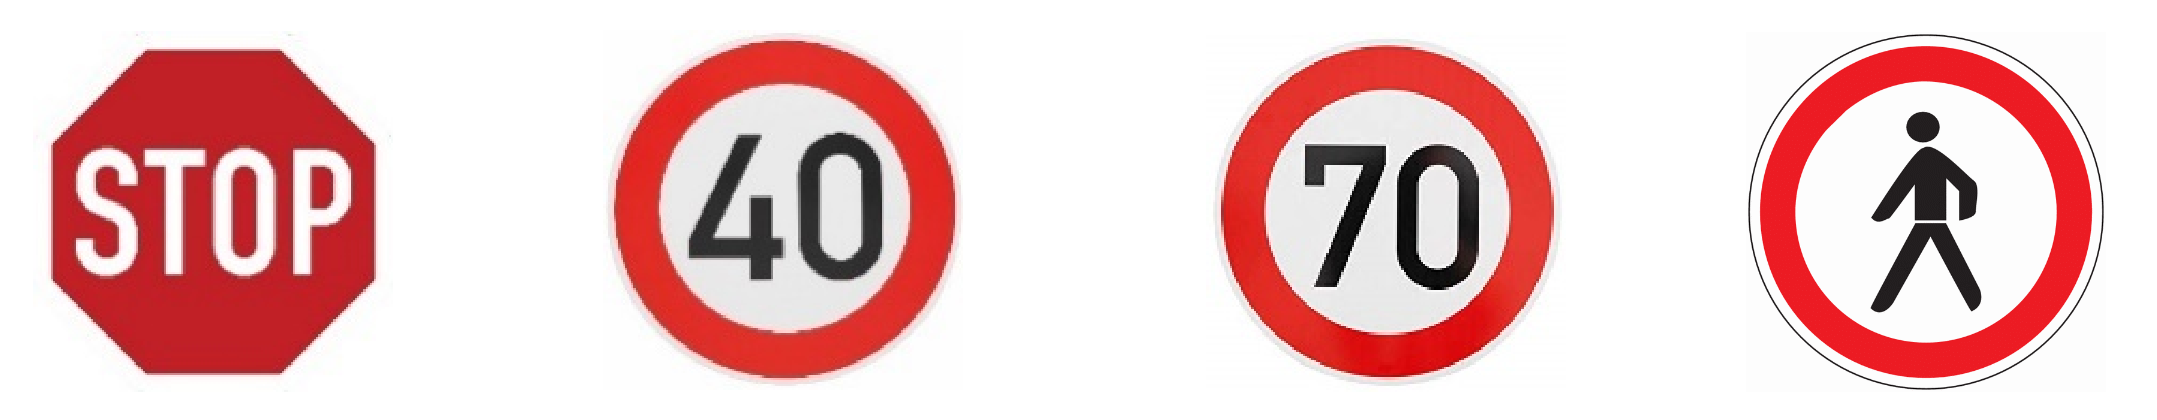
\includegraphics[width=0.9\textwidth]{images/Verkehrszeichen}
	\caption{Verkehrszeichen}
	\label{fig:verkehrszeichen}
\end{figure}

\subsection{Implementierung}
Um diese Motivation umsetzen zu k"onnen, haben wir ein k"unstliches neuronales Netz gew"ahlt. Dieses ist biologischen Prozessen nachempfunden und wird vermehrt im Bereich des maschinellen Lernen von Bildern verwendet. Das neuronale Netzwerk YOLO (You Only Look Once \cite{darknet13}) ist ein State-of-the-art real-time Objektdetektor
%TODO: dieses "state-of-the-art" ist eigentlich nur ein Kampfbegriff für "neuster Stand" und sagt m.Mn. nach nichts über die Technologie aus (Frederic)
basierend auf dem \textbf{Darknet} , ein Machine Learning Framework basierend auf C und CUDA.
%TODO: Darknet kurz erklären (Frederic) @edit DP
Die allgemeine Herausforderung eines Objektdetektors besteht darin, das Objekt im Bild zu detektieren und anschliessend zu klassifizieren. Der Vorteil des YOLO Netzes besteht neben der gleichzeitigen Lokalisierung \& Klassifizierung mehrerer Objekte in einem Bild, dass es auf unerwartete Eingaben sehr adaptiv reagiert und somit f"ur weniger Ausf"alle des Erkennungssystems sorgt. Dies erm"oglicht uns auch mehrere Verkehrsschilder auf einmal in einem Bild zu erkennen, wobei das aktuell n"achstgelegene Schild selektiert wird.

Der erste von uns verwendete Ansatz war die Benutzung der aktuellen Version YOLOv3. Es stellte sich jedoch heraus, dass die eingeschr"ankte Hardware auf dem Fahrzeug der limitierende Faktor ist und der ROS Wrapper nicht das aktuelle YOLOv3 verwenden kann. Daher wurde aus Gr"unden der Performance die YOLOv2 Tiny Version verwendet, welche eine reduzierte Variante des YOLOv2 darstellt und eine geringere Pr"azision in der Erkennung hat.

\subsection{Aufbau des neuronalen Netzes}
\label{sec:cnn_aufbau}
Ein k"unstliches neuronales Netz besteht aus mehreren Neuronen, die "uber mehrere Schichten (Layer) mit einander verbunden sind (siehe Abb \ref{fig:neunet}). YOLO ist ein Single CNN (Convolution Neuronal Network, faltende neurale Netze),
%TODO: wenn so ein Begriff eingeführt wird, sollte er eigentlich auch (zumindest kurz) erläutert werden (Frederic) @edit DP
welches aufgrund seines schlanken Aufbaus eine enorme Schnelligkeit erm"oglicht. Es verarbeitet ein Bild und detektiert dabei mehrere Objekte (Single Shot Detector). Andere Netze ben"otigen f"ur diese vergleichbare Detektion mehrere Durchl"aufe - jeweils einen Durchlauf f"ur das Detektieren der Objekte und jeweils eine Iteration pro gefundenem Objekt zur Klassifikation (z.B. R-CNN, R-FCN).
%TODO: Referenzen (Frederic)

\begin{figure}[h]
	\centering
	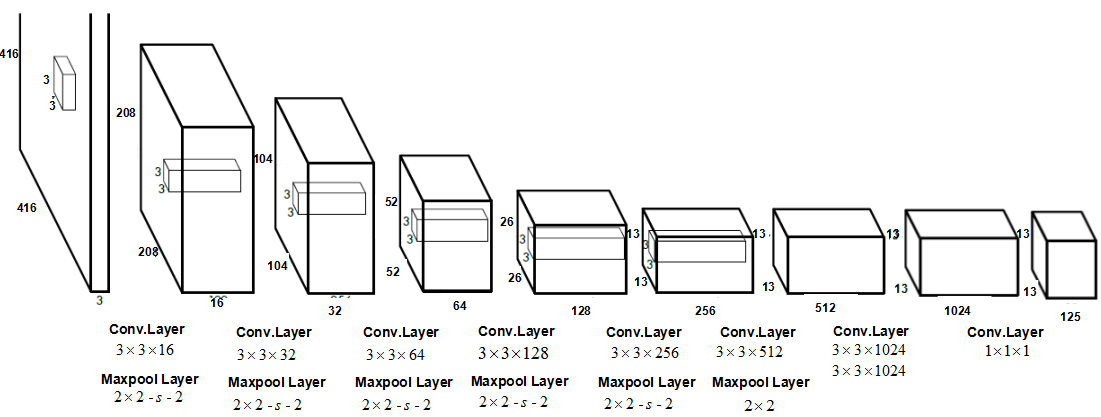
\includegraphics[width=0.90\textwidth]{images/aufbauskizze}
	\caption{Aufbauskizze}
	\label{fig:neunet}
\end{figure}

Das YOLO CNN besteht aus mehreren Convolution und Maxpool Layers zum subsampling.
%TODO: "Convolution", "Maxpool Layers", "subsampling" -> alles Begriffe, mit denen der Leser in aller Regel nichts direkt anfangen kann (Frederic) @ edit DP Subsampling zum herunterskalieren, 
Diese reduzieren die Dimension der Eingabedarstellung mit Hilfe von Annahmen,
%TODO: was für "Annahmen"? -> das muss erklärt werden! (Frederic)
so dass der Rechenaufwand erheblich reduziert wird. Am Ende befindet sich ein $16*16*14$ Quader, der die Klassifikation und Detektion des verarbeiteten Inputs "ubernimmt. Wof"ur stehen diese Dimensionen?
%TODO: "Wofür stehen diese Dimensionen" -> ist eine Frage, kann hier nicht so mit Doppelpunkt verwendet werden (Frederic) @edit DP

Das 16 x 16 Grid beschreibt die Gr"osse eines Rasters, in das das Bild unterteilt wird. Die Tiefe 14 l"asst sich in zwei Werte aufteilen. Zum einen die Startposition der Boundingbox sowie dessen H"ohe und Breite (x,y).  Zum anderen die IoU (Intersection over Union). Dieser Wert gibt das Verh"altnis zwischen der "uberlappenden Fl"ache und der vereinigten Fl"ache an. Veranschaulicht ist dies ein Ma\ss \ daf\"ur, wie gut eine Detektion mit der realen Position des Objekts vergleichbar ist (siehe Abb. \ref{fig:stoppschild}). Das neuronale Netz berechnet den IoU-Wert und gibt somit ihre Treffergenauigkeit an. Die Anzahl unserer 4 Objektklassen (STOP, Fussg"anger, 40, 70),  werden der Tiefe des Quaders noch hinzuaddiert,
%TODO: was sind (unsere) "Objektklassen"? Was is die "Tiefe"? (Frederic) @edit DP
sodass der Quader nachfolgende Gr"osse besitzt:

%TODO: ZUM ABSCHNITT: Das klingt gerade alles für mich noch sehr schwammig, es werden haufenweise Begriffe eingeführt, die man als Fachfremder (jemand, der nichts mit neuronalen Netzwerken zu tun hat) nicht versteht... Z.B. die "Tiefe" bzw. der Begriff "Quader" kommen ohne Zusammenhang. (Frederic)
%TODO: Ich würde entweder alles viel detaillierter erklären oder das meiste rausschmeißen und die Beschreibung des neuronalen Netzes stattdessen ganz allgemein und einfach halten. (Frederic)

\begin{equation}
\begin{bmatrix}16 * 16 (Grid)\end{bmatrix} * \begin{bmatrix}2 * 5 + 4 (Objektklassen)\end{bmatrix}
\end{equation}

\begin{figure}[h]
	\centering
	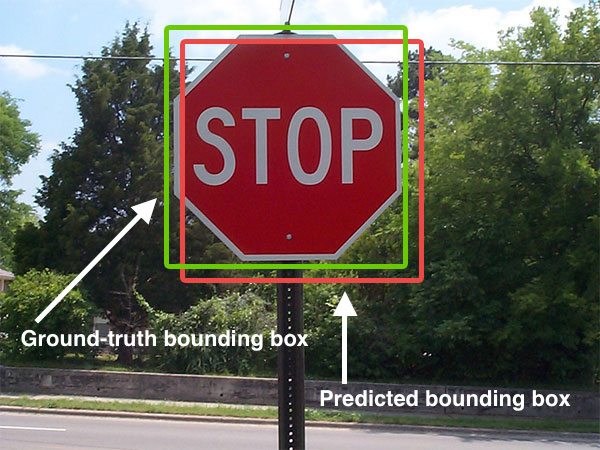
\includegraphics[width=0.65\textwidth]{images/stoppschild}
	\caption{Erkanntes Stoppschild mit Boundingboxes}
	\label{fig:stoppschild}
\end{figure}

\subsection{Ablauf der Detektion}

\begin{figure}[h]
	\centering
	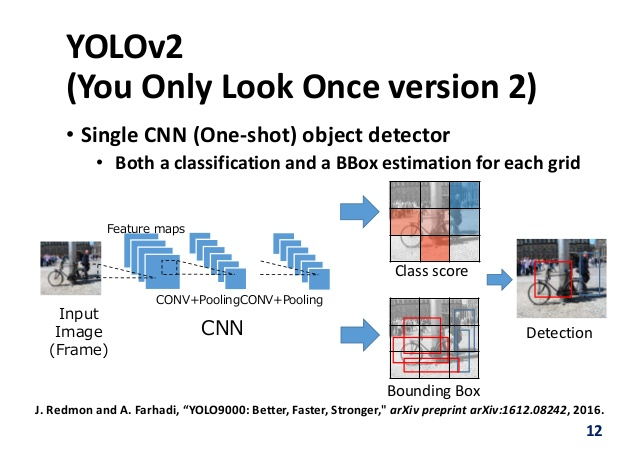
\includegraphics[width=0.9\textwidth,trim={1.2cm 1cm 1cm 6.3cm},clip]{images/yolo_schaubild}
	\caption{Ablaufprozess des neuronalen Netzes YOLO}
	\label{fig:yolo}
\end{figure}

Die einzelnen Frames der Webcam werden dem neuronalen Netz als Input zur Verf"ugung gestellt. Somit verwendet das YOLO Netz ein vollst"andiges Bild zur Erkennung, das es uns erm"oglicht, weniger Hintergrundfehler zu erhalten. Au\ss erdem wird der Kontext der Objekte mitbetrachtet. Das gesamte Bild wird in einzelne Grids aufgeteilt und dem CNN "ubergeben. Pro Grid kann ein Objekt erkannt werden. Damit man auch mehrere Objekte detektieren kann, die eventuell weiter entfernt sind, verwenden wir abweichend vom Standard Grid (32 x 32) eine Gr"osse von 16 x 16 Pixel. Der komplexe Prozess des CNN l"asst sich vereinfacht durch diesen Ablauf beschreiben:

\begin{enumerate}
	\item Bildinput wird auf Eingangsgr"o\ss e des Netzes angepasst (416 x 416 Pixel)
	\item Durchlaufen des Convolutional Network
	\item Non-max Suppression (Pro Objektregion wird das Objekt nur einmal erkannt, reduziert Redundanzen) 
\end{enumerate}

Das detektierte Objekt mit der h"ochsten "Ubereinstimmung (> 60\%) mit unseren Objektklassen wird im Bild durch eine bunte Boundingbox gekennzeichnet und dem entsprechenden Label versehen.

\begin{figure}[h]
	\centering
	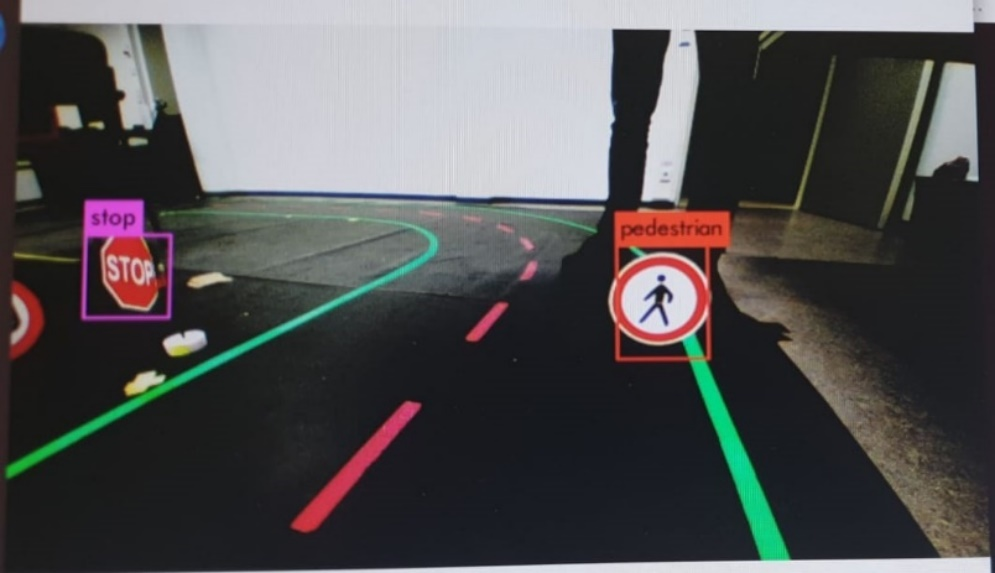
\includegraphics[width=0.9\textwidth,trim={0.5cm 1cm 1cm 1cm},clip]{images/boundingboxes}
	\caption{Erkannte und markierte Schilder auf dem Rundkurs}
	\label{fig:boundingboxes}
\end{figure}

Anschlie\ss end wird das Ergebnis der Verkehrsschildererkennung "uber das ROS-Netzwerk gepublished. Um das YOLO Netz auf dem Fahrzeug auszuf"uhren verwenden wir ein angepasstes Interface von leggedrobotics \cite{leggedrobotics}. Es l"adt die Bilder der ROS-Node \texttt{webcam\_publisher} ein und startet die Verkehrsschildererkennung mit dem selbsttrainierten Netzwerk "uber ROS. "Uber das ROS Netzwerk k"onnen nun die Anzahl der erkannten Objekte (Topic: \texttt{object\_detector}), die Position dieser (Topic: \texttt{bounding\_boxes}, ein Array mit Boundingboxen in Pixelkoordinaten) und das resultierende Bild mit den erkannten Detektionen (Topic: \texttt{detection\_image}) ausgelesen werden.

\subsection{Training}

Das Neuronale Netz wurde bereits mit dem VOC Datensatz
%TODO: was ist "VOC"? -> erklären, kennt der Leser nicht (Frederic)
per Transfer Learning (Die Ergebnisse eines fertig trainierten Netzes werden auf ein neues Netz "ubertragen. Die Layer /Neuronen des Netzes werden nun mit dem neuen Datenset trainiert.) vorverarbeitet.
%TODO: schlechter Stil, hier in Klammern ganze Sätze einzuschieben und danach den vorherigen Satz noch zu beenden, verstehe nicht, was gemeint sein soll (Frederic)
Dies erm"oglichte es uns, ein vortrainiertes Netz zu verwenden, welches bereits f"ur die Objekterkennung konfiguriert ist und durch unseren Datensatz optimiert wird. Wir haben das Netz mit dem Supervised-Learning-Verfahren trainiert (ein "uberwachtes Lernen, bei dem die Ergebnisse des Lernprozesses mit den Referenzergebnissen verglichen werden).  Zu diesem Zweck wurde der Datensatz in Trainings- und Testdaten aufgeteilt. Unser Datensatz besteht aus 1700 selbstaufgenommenen Verkehrsschildern "uber die Webcam des Autos, ca. 400 Bilder pro Objektklasse (STOP, Fussg"anger, 40, 70), die mit dem Tool Yolo\_mark \cite{Yolo_mark} gelabelt wurden.

Der Trainingsdatensatz wird als Input f"ur das Netz verwendet. Diese passieren das Netz "uber die Neuronen durch die verschiedenen Layer zum Output Quader (Forward Pass). Das Ergebnis der Berechnung wird mit dem bekannten Ergebnis des Testdatensatzes verglichen und der Fehler/Abweichung berechnet. Dieser Fehler wird durch das Netzwerk r"uckw"arts propagiert (Backward Pass) und jedes Neuron entsprechend im Verh"altnis zur Learning Rate (0,001) angepasst. Somit wird das Netz nur minimal ver"andert, um ein Overshooting (zu gro\ss e Ver"anderungen, z.B. bei einer Fehlfunktion) zu verhindern. Dieser Ablauf beschreibt eine Trainings-Epoche des Netzes.  Solch eine Epoche wird zum Trainieren mehrere 1000 Mal ausgef"uhrt um ein zufriedenstellendes Ergebnis des Trainings zu erhalten. (Darauf wird in folgendem Abschnitt noch genauer eingegangen.) Das verwendete Darknet YOLO Datenset besteht aus nachfolgenden Elementen:

\begin{itemize}
	\item \textbf{.cfg} enth"alt die Strukturdefinition des neuronalen Netzes (Layers, Gr"osse des Inputs, Gridgr"osse, Learningrate, ...)
	\item \textbf{.weights} enth"alt die erlernten Gewichte
	\item \textbf{.yaml} Referenzfile zu den Weights und Config, inklusive Erkennungsrate (Threshold)
	\item \textbf{.data} Referenzfile zu Trainingsdaten \& Beschriftung
\end{itemize}

\subsection{Validierung}
Die G"ute/Genauigkeit der richtigen Detektion eines Objektes wird durch folgende Werte bestimmt:

\begin{figure}[h]
	\centering
	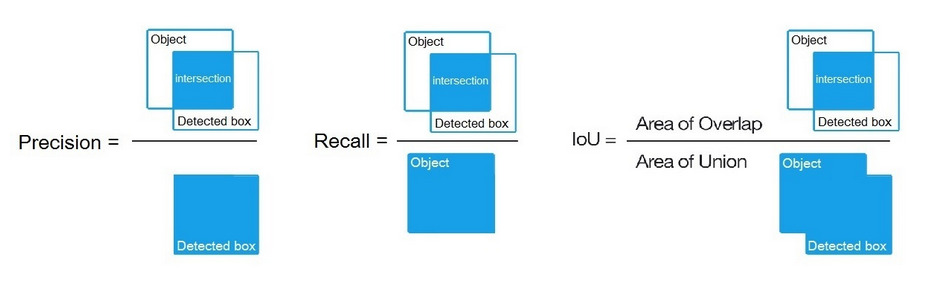
\includegraphics[width=1.0\textwidth]{images/genauigkeit}
	\caption{G"utebestimmung}
	\label{fig:genauigkeit}
\end{figure}

Die Detektionsfl"ache wird mit der tats"achlichen Fl"ache eines Objektes vergleichen und der Grad der "Ubereinstimmung bestimmt. W"ahrend des Trainings kann man in Abb. \ref{fig:training} erkennen, dass neben dem rapide absinkenden Fehler (Loss) in blau, der mAP-Wert (mean average precision) in rot, mit Laufe der Iterationen stetig steigt und sich der 100\% Linie ann"ahert (Convergence). Ab ca. 93\% schwankt der Wert immer mehr und n"ahert sich dem Wert 1 an. Dieser Bereich unterscheidet sich signifikant vom restlichen Graphen und deutet auf Overfitting hin.

Overfitting beschreibt das Problem, dass ein Netz beim Trainieren alle bereits bekannten Bilder sehr oft als Input erhalten hat und diese eher auswendig lernt anstatt des Konzepts des Bildes zu lernen. Um dieses ungewollte Verhalten zu minimieren werden beim Training in jedem Layer des Netzwerks eine gewisse Anzahl an Neuronen ausgelassen (Dropout). Zus"atzlich werden die Bilder in einem Trainingsdatenset und Testdatenset aufgeteilt mit dem Verh"altnis 70 zu 30.
%TODO: was ist das für ein Verhältnis bzw. was gibt das an? (Frederic)

\begin{figure}[h]
	\centering
	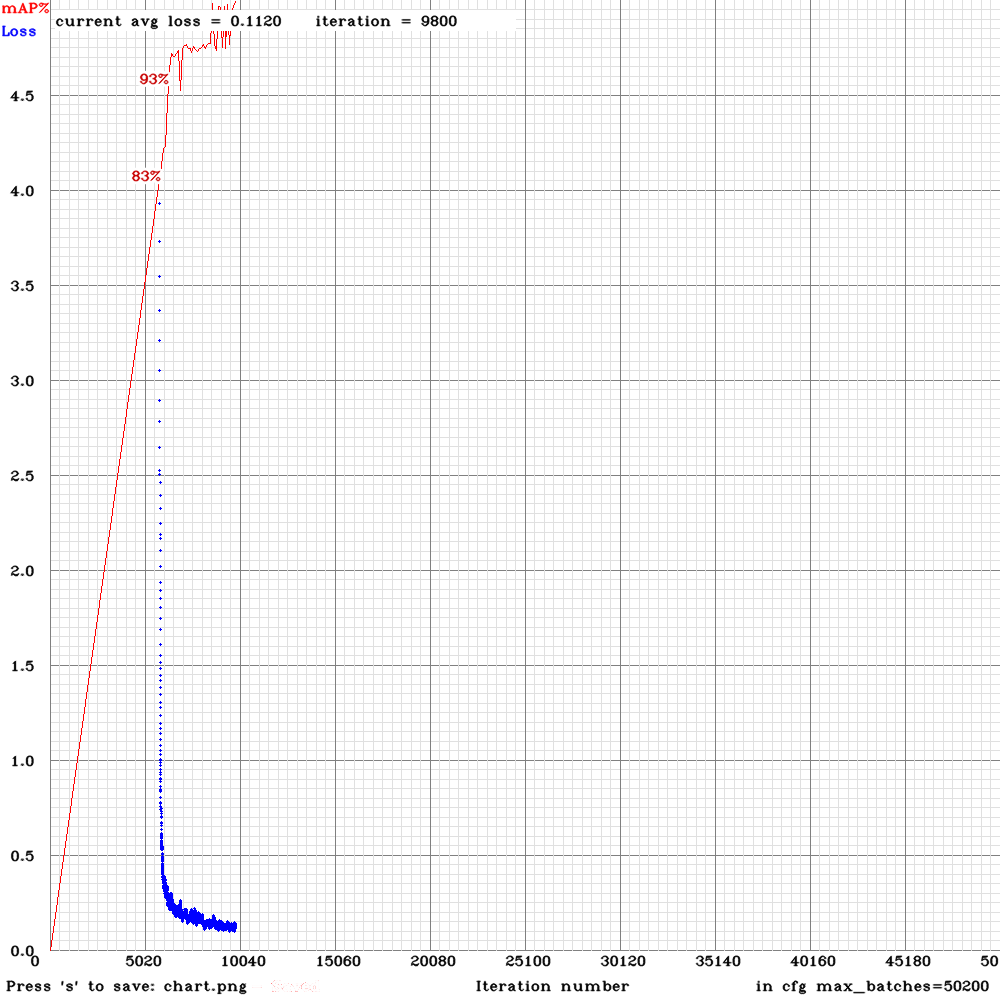
\includegraphics[width=0.85\textwidth]{images/training}
	\caption{Trainingsverlauf}
	\label{fig:training}
\end{figure}

Nach dem Training k"onnen wir die jeweiligen Objektklassen (STOP, Fussg"anger, 40, 70) mit einer Wahrscheinlichkeit von 90\% bzw. bei dem Schild 70 mit 77\% richtig erkennen. Der IoU (siehe Abschnitt \ref{sec:cnn_aufbau}) Wert liegt bei 63\% und der mAP bei 87\%. (Siehe Abb. \ref{fig:ergebnis}).

\begin{figure}[ht]
	\centering
	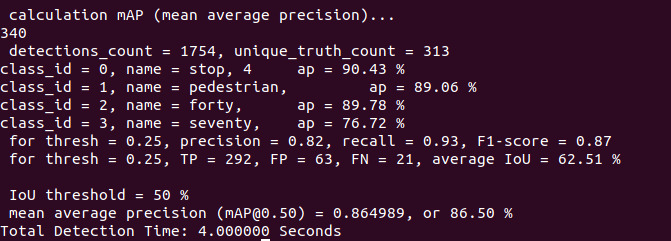
\includegraphics[width=0.9\textwidth]{images/ergebnis}
	\caption{Ergebnisse des Trainings}
	\label{fig:ergebnis}
\end{figure}

\subsection{Optimierungen}
Im zuk\"unftigen Versionen wird der ROS-Wrapper in der Lage sein mit der aktuellen Yolov3 Version interagieren zu k"onnen, sodass wir eine noch schnellere, pr"azisere und ressourcenschonendere Verkehrsschilderkennung verwenden k"onnen.

Die Genauigkeit der Schildererkennung kann durch den Datensatz von 1000 gelabelten Bildern pro Klasse verbessert werden.

Die allgemeine Leistungssteigerung der Fahrzeughardware w"urde die Erkennung von vielen weiteren digitalen bzw. dynamischen Schildern erm"oglichen, sodass das Fahrzeug auch in Baustellsituationen entsprechend reagieren kann.
%TODO: was für "digitale" bzw. "dynamische" Schilder? (Frederic)
%TODO: warum gerade "Baustellsituationen"? würde ich eher weglassen (Frederic)

\begin{figure}[ht]
	\centering
	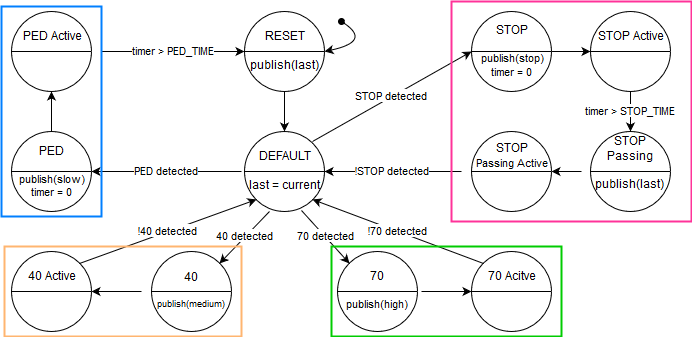
\includegraphics[width = 1\textwidth]{images/StateMachine.png}
	\caption{Zustandsautomat f\"ur die Schildererkennung}
	\label{fig:zustandsautomat}
\end{figure}

\subsection{Reaktion auf erkannte Schilder}
Momentan erkennt das neuronale Netz vier Schilder, doch das Roboterauto reagiert noch nicht auf diese und erkennt sie nur. Das Team hat bereits einen Zustandsautomaten f\"ur die Weiterverarbeitung der Schildererkennung entwickelt (siehe Abbildung \ref{fig:zustandsautomat}) und in C++ realisiert.

Wenn das neuronale Netz ein Schild oder mehrere Schilder erkennt, dann werden diese \"uber ein ROS-Topic ver\"offentlicht. Diese erkannten Schilder werden zun\"achst darauf \"uberpr\"uft, welches das n\"achste Schild im Abstand zum Roboterauto ist und ob der Abstand zu dem Schild klein genug ist, um darauf reagieren zu m\"ussen. Falls dies der Fall ist, so wird das entsprechend n\"achste Schild als Ereignis an den Zustandsautomaten weitergegeben, falls nicht wird das Ereignis weitergegeben, dass kein Schild erkannt wurde.
\\\\Die Bedeutungen der einzelnen K\"urzel des Zustandsautomaten werden nachfolgend erkl\"art:
\begin{itemize}
	\item Geschwindigkeitenereignisse werden mit den Konstanten \textbf{\textit{stop}}, \textbf{\textit{slow}}, \textbf{\textit{medium}} und \textbf{\textit{high}} beschrieben, wobei gilt:
	\begin{align}
	\begin{split}
	\label{vel_vergleich}
	0 = stop < slow < medium < high
	\end{split}
	\end{align}
	
	\item \textbf{\textit{current}} und \textbf{\textit{last}} sind Variablen und beschreiben, welches Geschwindigkeitsereignis gerade in diesem Moment und welches Geschwindigkeitsereignis zuvor galt. Beide haben den Initialwert \textbf{\textit{medium}}.
	
	\item Die Funktion \textbf{\textit{publish(x)}} ver\"offentlicht ein Geschwindigkeitsereignis \"uber ein ROS-Topic, welches dann von anderen ROS-Nodes abonniert werden kann.
	
	\item Die Zeitkonstanten \textbf{\textit{PED\underline{\ }TIME}} und \textbf{\textit{STOP\underline{\ }TIME}} stellen einen Zeitwert in Sekunden dar.
	
	\item \textbf{\textit{timer}} ist ein Z\"ahler und z\"ahlt die Sekunden hoch.
	
	\item \textbf{\textit{STOP}}, \textbf{\textit{PED}}, \textbf{\textit{40}} und \textbf{\textit{70}} sind Schildereignisse, welche der Zustandsautomat als Eingabe empf\"angt. 
	
	\item Die Transitionsbedingung \textbf{\textit{x detected}} schaltet dann, wenn das entsprechende Schildereignis von dem Zustandsautomaten als Eingabe empfangen wurde.
	
	\item Der Zustand \textbf{\textit{RESET}} stellt den Initialzustand dar und ver\"offentlicht das Geschwindigkeitsereignis \textbf{\textit{last}}.
	
	\item Der Zustand \textbf{\textit{DEFAULT}} ist ein Zustand, welcher in jedem Ereigniszyklus einmal ausgel\"ost wird und das Geschwindigkeitsereignis \textbf{\textit{current}} auf \textbf{\textit{last}} setzt.
	
\end{itemize}


\begin{figure}[h]
	\begin{minipage}[t]{4cm}
		\vspace{0pt}
		\centering
		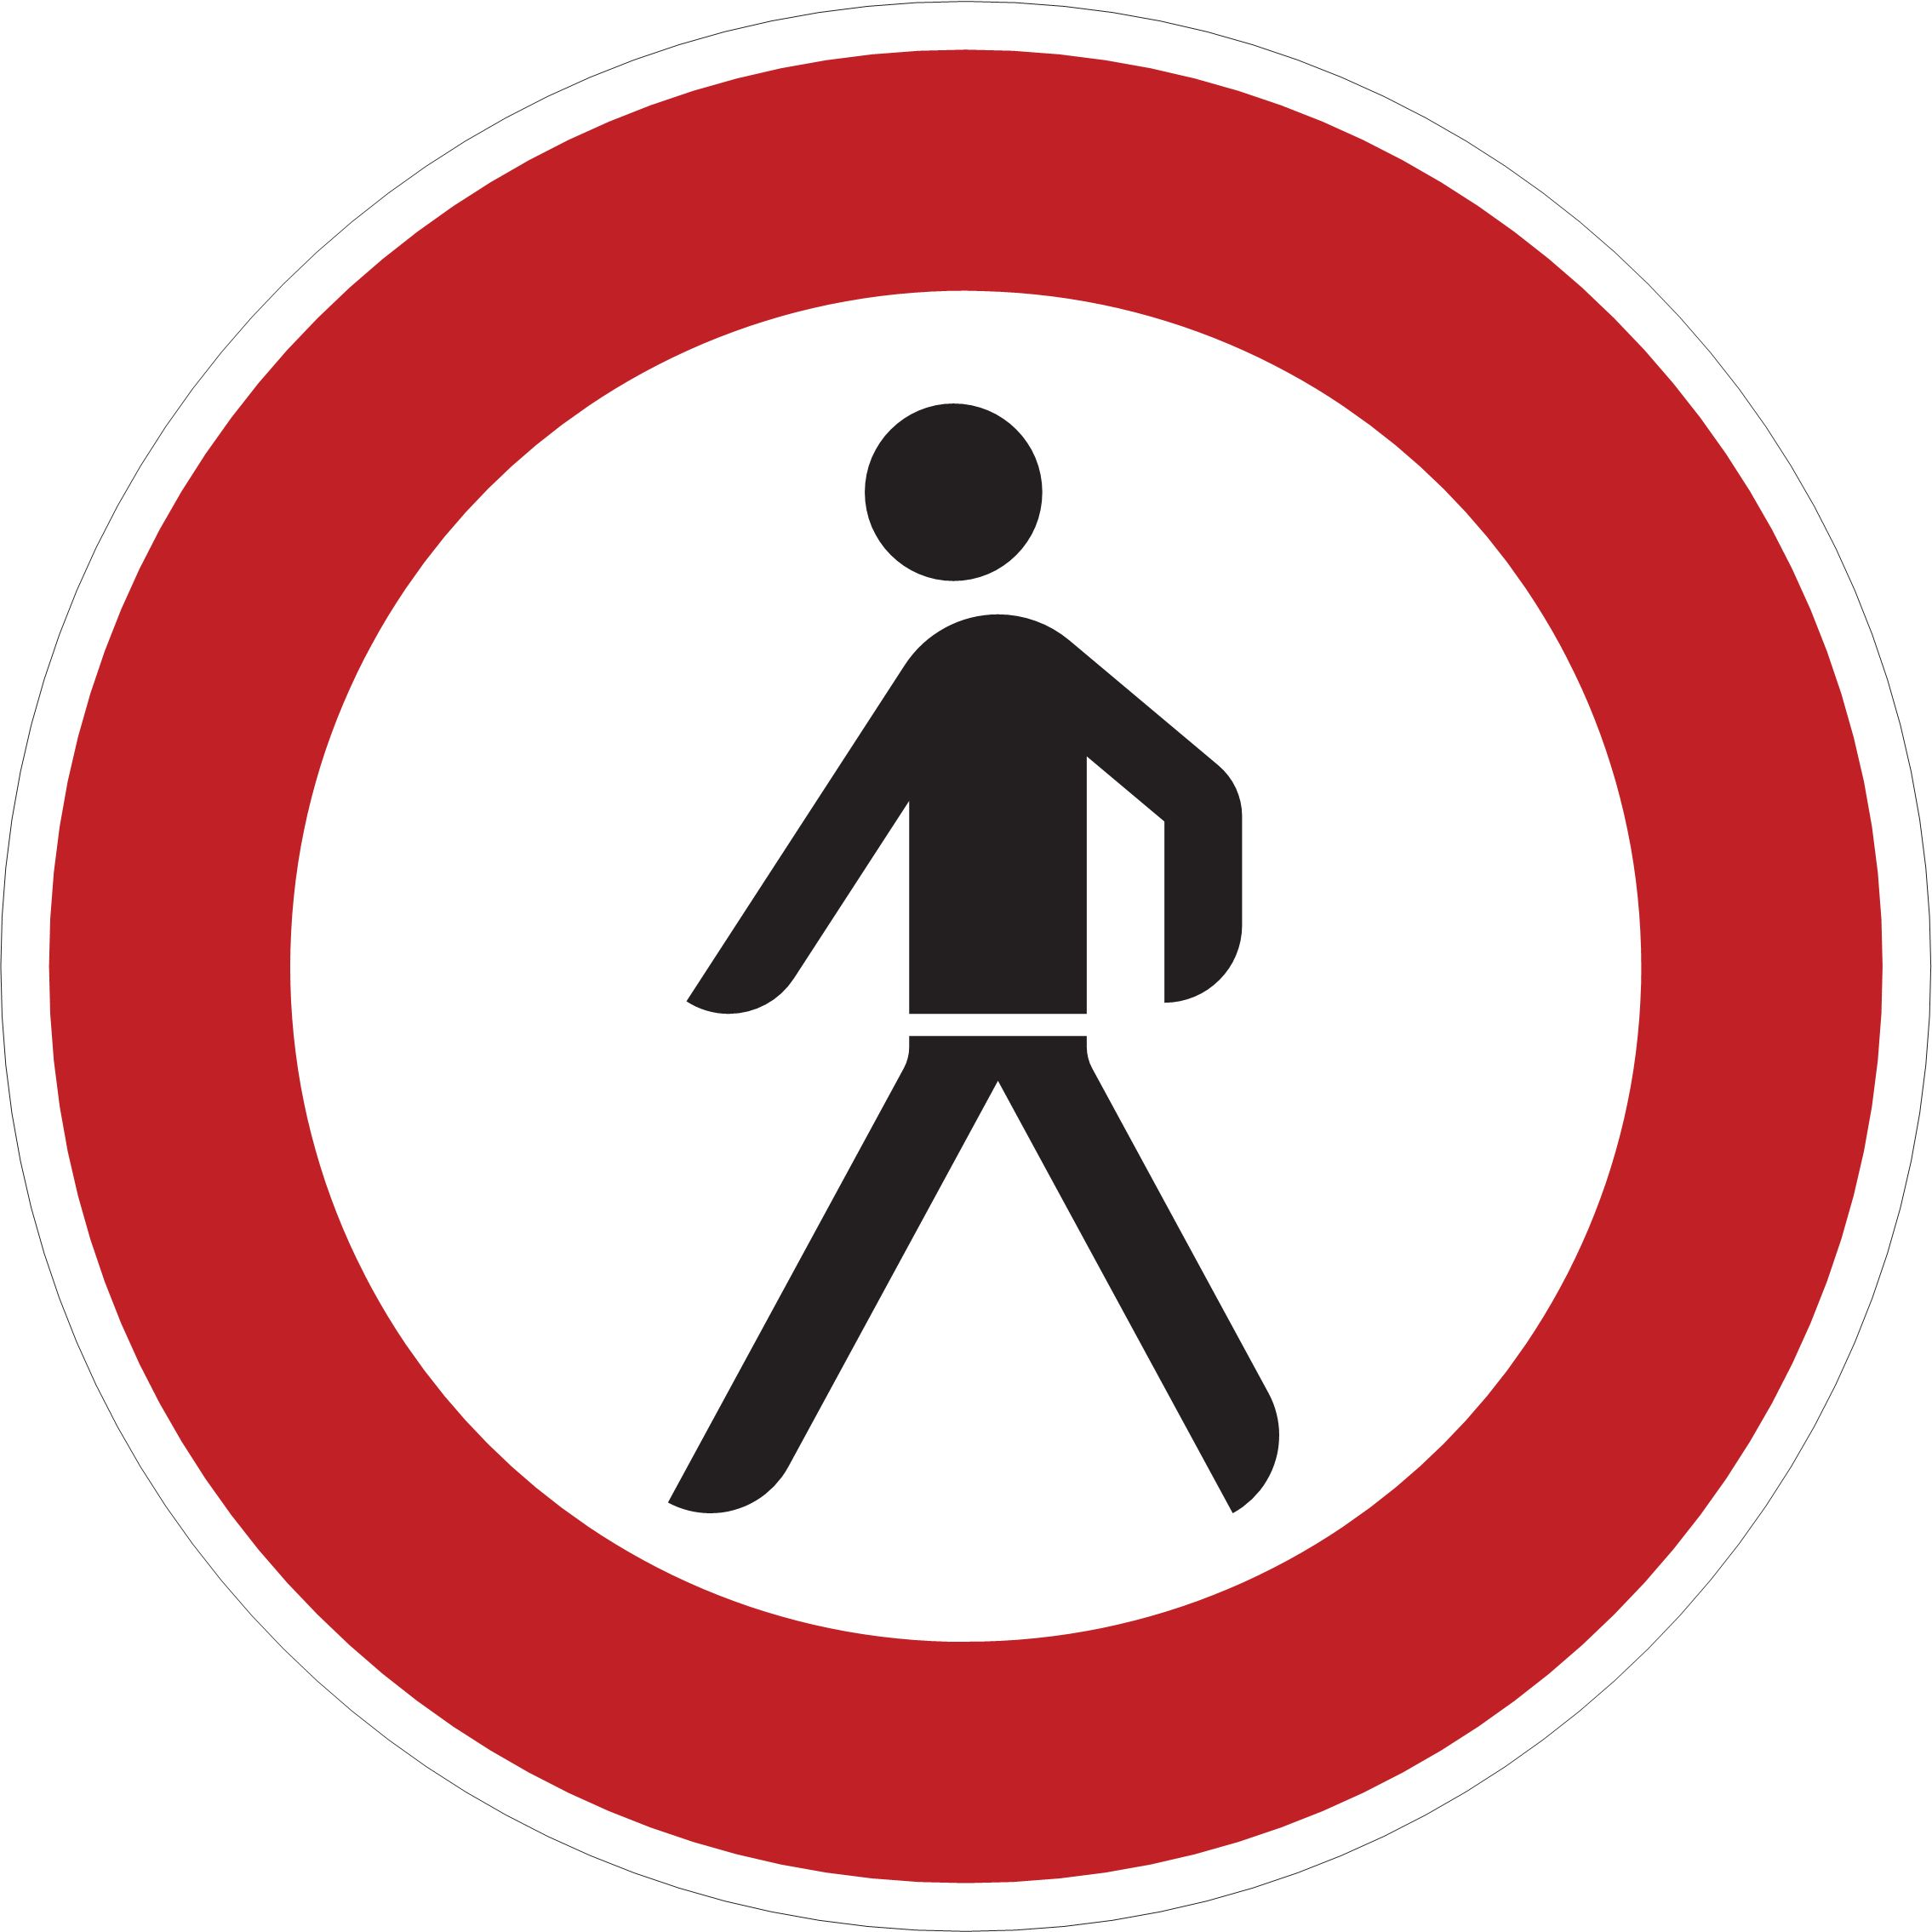
\includegraphics[scale=0.07]{images/PED.jpg}
		\caption{Verbot f\"ur Fu\ss{}g\"anger}
		\label{fig:PED}
	\end{minipage}
	\hfill
	\begin{minipage}[t]{10cm}
		\vspace{0pt}
		\begin{itemize}
			\item Der blau markierte Bereich im Zustandsautomaten beschreibt, was das Schild \glqq Verbot f\"ur Fu\ss{}g\"anger\grqq \ bewirkt. Das Schild wird als "Vorsicht Fu\ss{}g\"anger"\  interpretiert.
			
			\item Wenn als Eingabe \textbf{\textit{PED}} empfangen wird, wird ein Z\"ahler gestartet und das Geschwindigkeitsereignis \textbf{\textit{slow}} ver\"offentlicht.
			
			\item Sobald der Z\"ahler \textbf{\textit{PED\underline{\ }TIME}} \"uberschritten wird, wird das Geschwindigkeitsereignis auf \textbf{\textit{last}} zur\"uckgesetzt und zur\"uck auf den Status \textbf{\textit{DEFAULT}} geschaltet.
		\end{itemize}
	\end{minipage}
\end{figure}


\begin{figure}[h]
	\begin{minipage}[t]{4cm}
		\vspace{0pt}
		\centering
		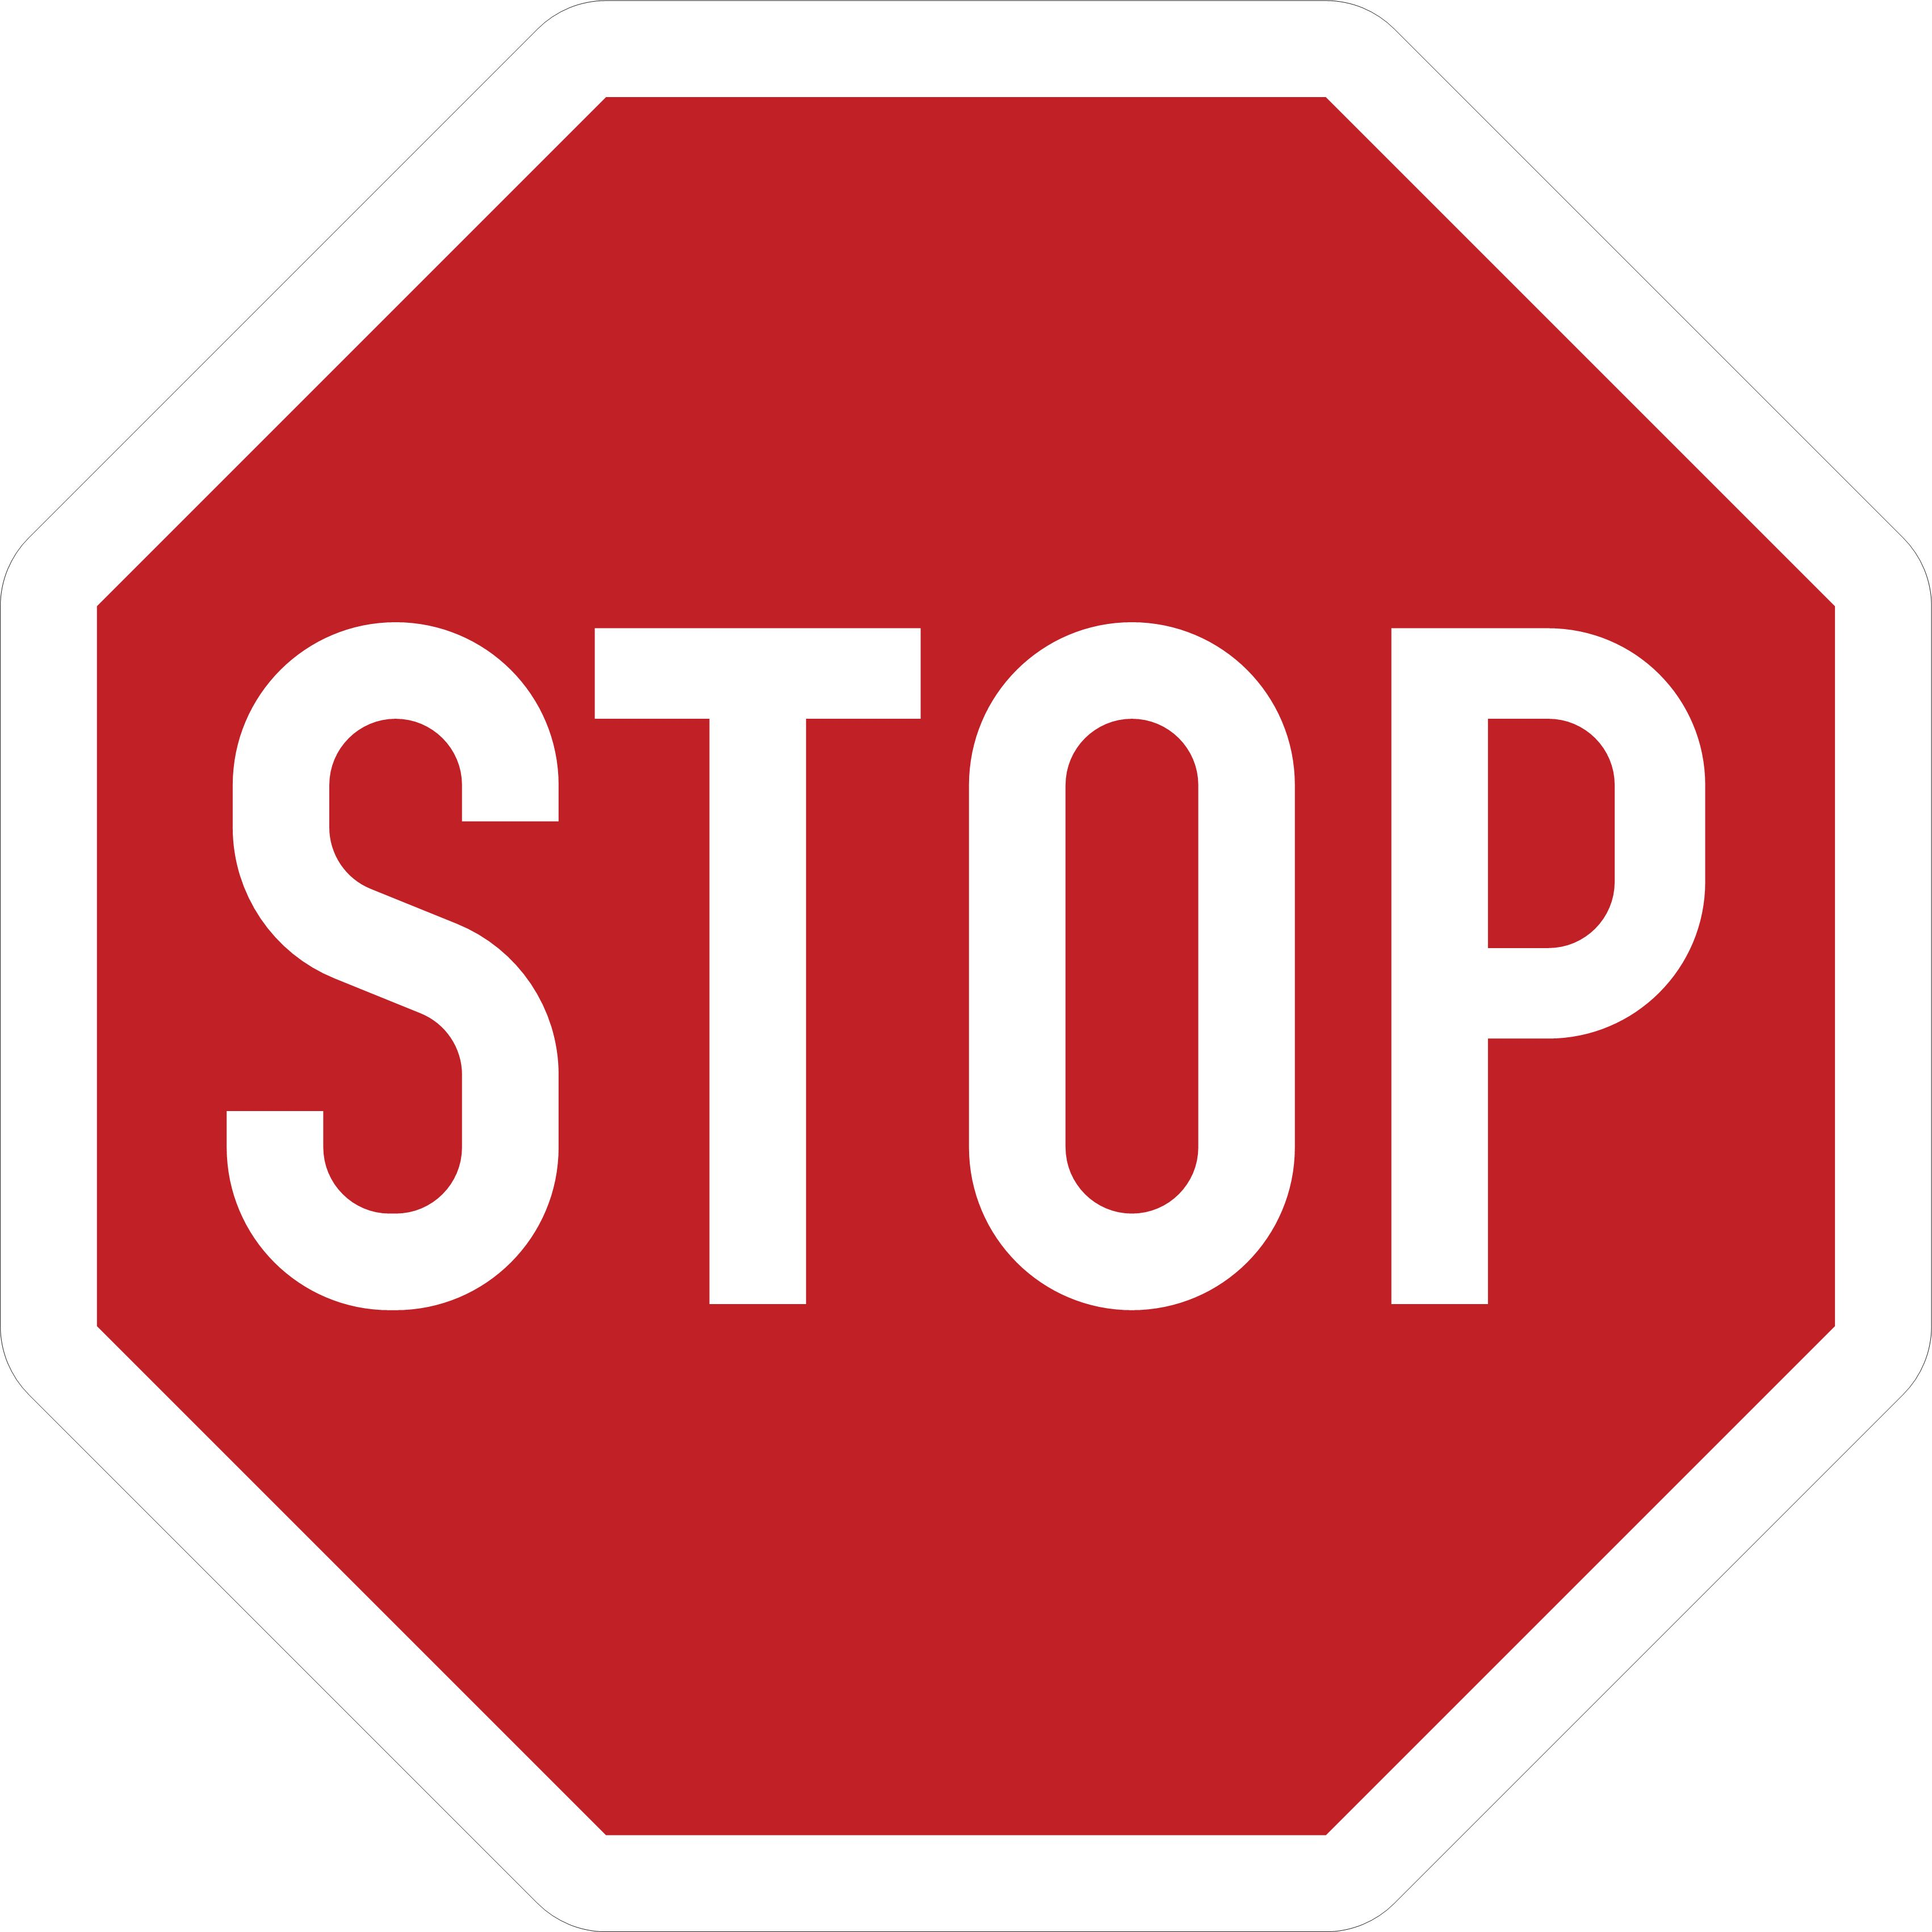
\includegraphics[scale=0.04]{images/STOP.jpg}
		\caption{Stoppschild}
		\label{fig:PED}
	\end{minipage}
	\hfill
	\begin{minipage}[t]{10cm}
		\vspace{0pt}
		\begin{itemize}
			\item Der magenta markierte Bereich im Zustandsautomaten beschreibt, was das Schild \glqq Stoppschild\grqq \ bewirkt.
			
			\item Wenn als Eingabe \textbf{\textit{STOP}} empfangen wird, wird ein Z\"ahler gestartet und das Geschwindigkeitsereignis \textbf{\textit{stop}} ver\"offentlicht.
			
			\item Sobald der Z\"ahler \textbf{\textit{STOP\underline{\ }TIME}} \"uberschritten wird, wird das Geschwindigkeitsereignis auf \textbf{\textit{last}} zur\"uckgesetzt. Hierbei wird darauf geachtet, dass der Zustandsautomat erst dann auf \textbf{\textit{DEFAULT}} weiterschaltet, wenn ein Ereignis au\ss{}er \textbf{\textit{STOP}} empfangen wird, um unendliche Schleifen zu vermeiden.
		\end{itemize}
	\end{minipage}
\end{figure}


\begin{figure}[h]
	\begin{minipage}[t]{4cm}
		\vspace{0pt}
		\centering
		
\includegraphics[scale=0.07]{images/40.png}
		\caption{Zul\"assige H\"ochstgeschw.}
		\label{fig:PED}
	\end{minipage}
	\hfill
	\begin{minipage}[t]{10cm}
		\vspace{0pt}
		\begin{itemize}
			\item Der orange markierte Bereich im Zustandsautomaten beschreibt, was das Schild \glqq Zul\"assige H\"ochstgeschwindigkeit 40km/h\grqq\ bewirkt.
			
			\item Wenn als Eingabe \textbf{\textit{40}} empfangen wird, wird das Geschwindigkeitsereignis \textbf{\textit{medium}} ver\"offentlicht.
			
			\item Sobald ein Geschwindigkeitsereignis au\ss{}er \textbf{\textit{40}} empfangen wird schaltet der Zustandsautomat zur\"uck auf den Status \textbf{\textit{DEFAULT}}
		\end{itemize}
	\end{minipage}
\end{figure}


\begin{figure}[h]
	\begin{minipage}[t]{4cm}
		\vspace{0pt}
		\centering
		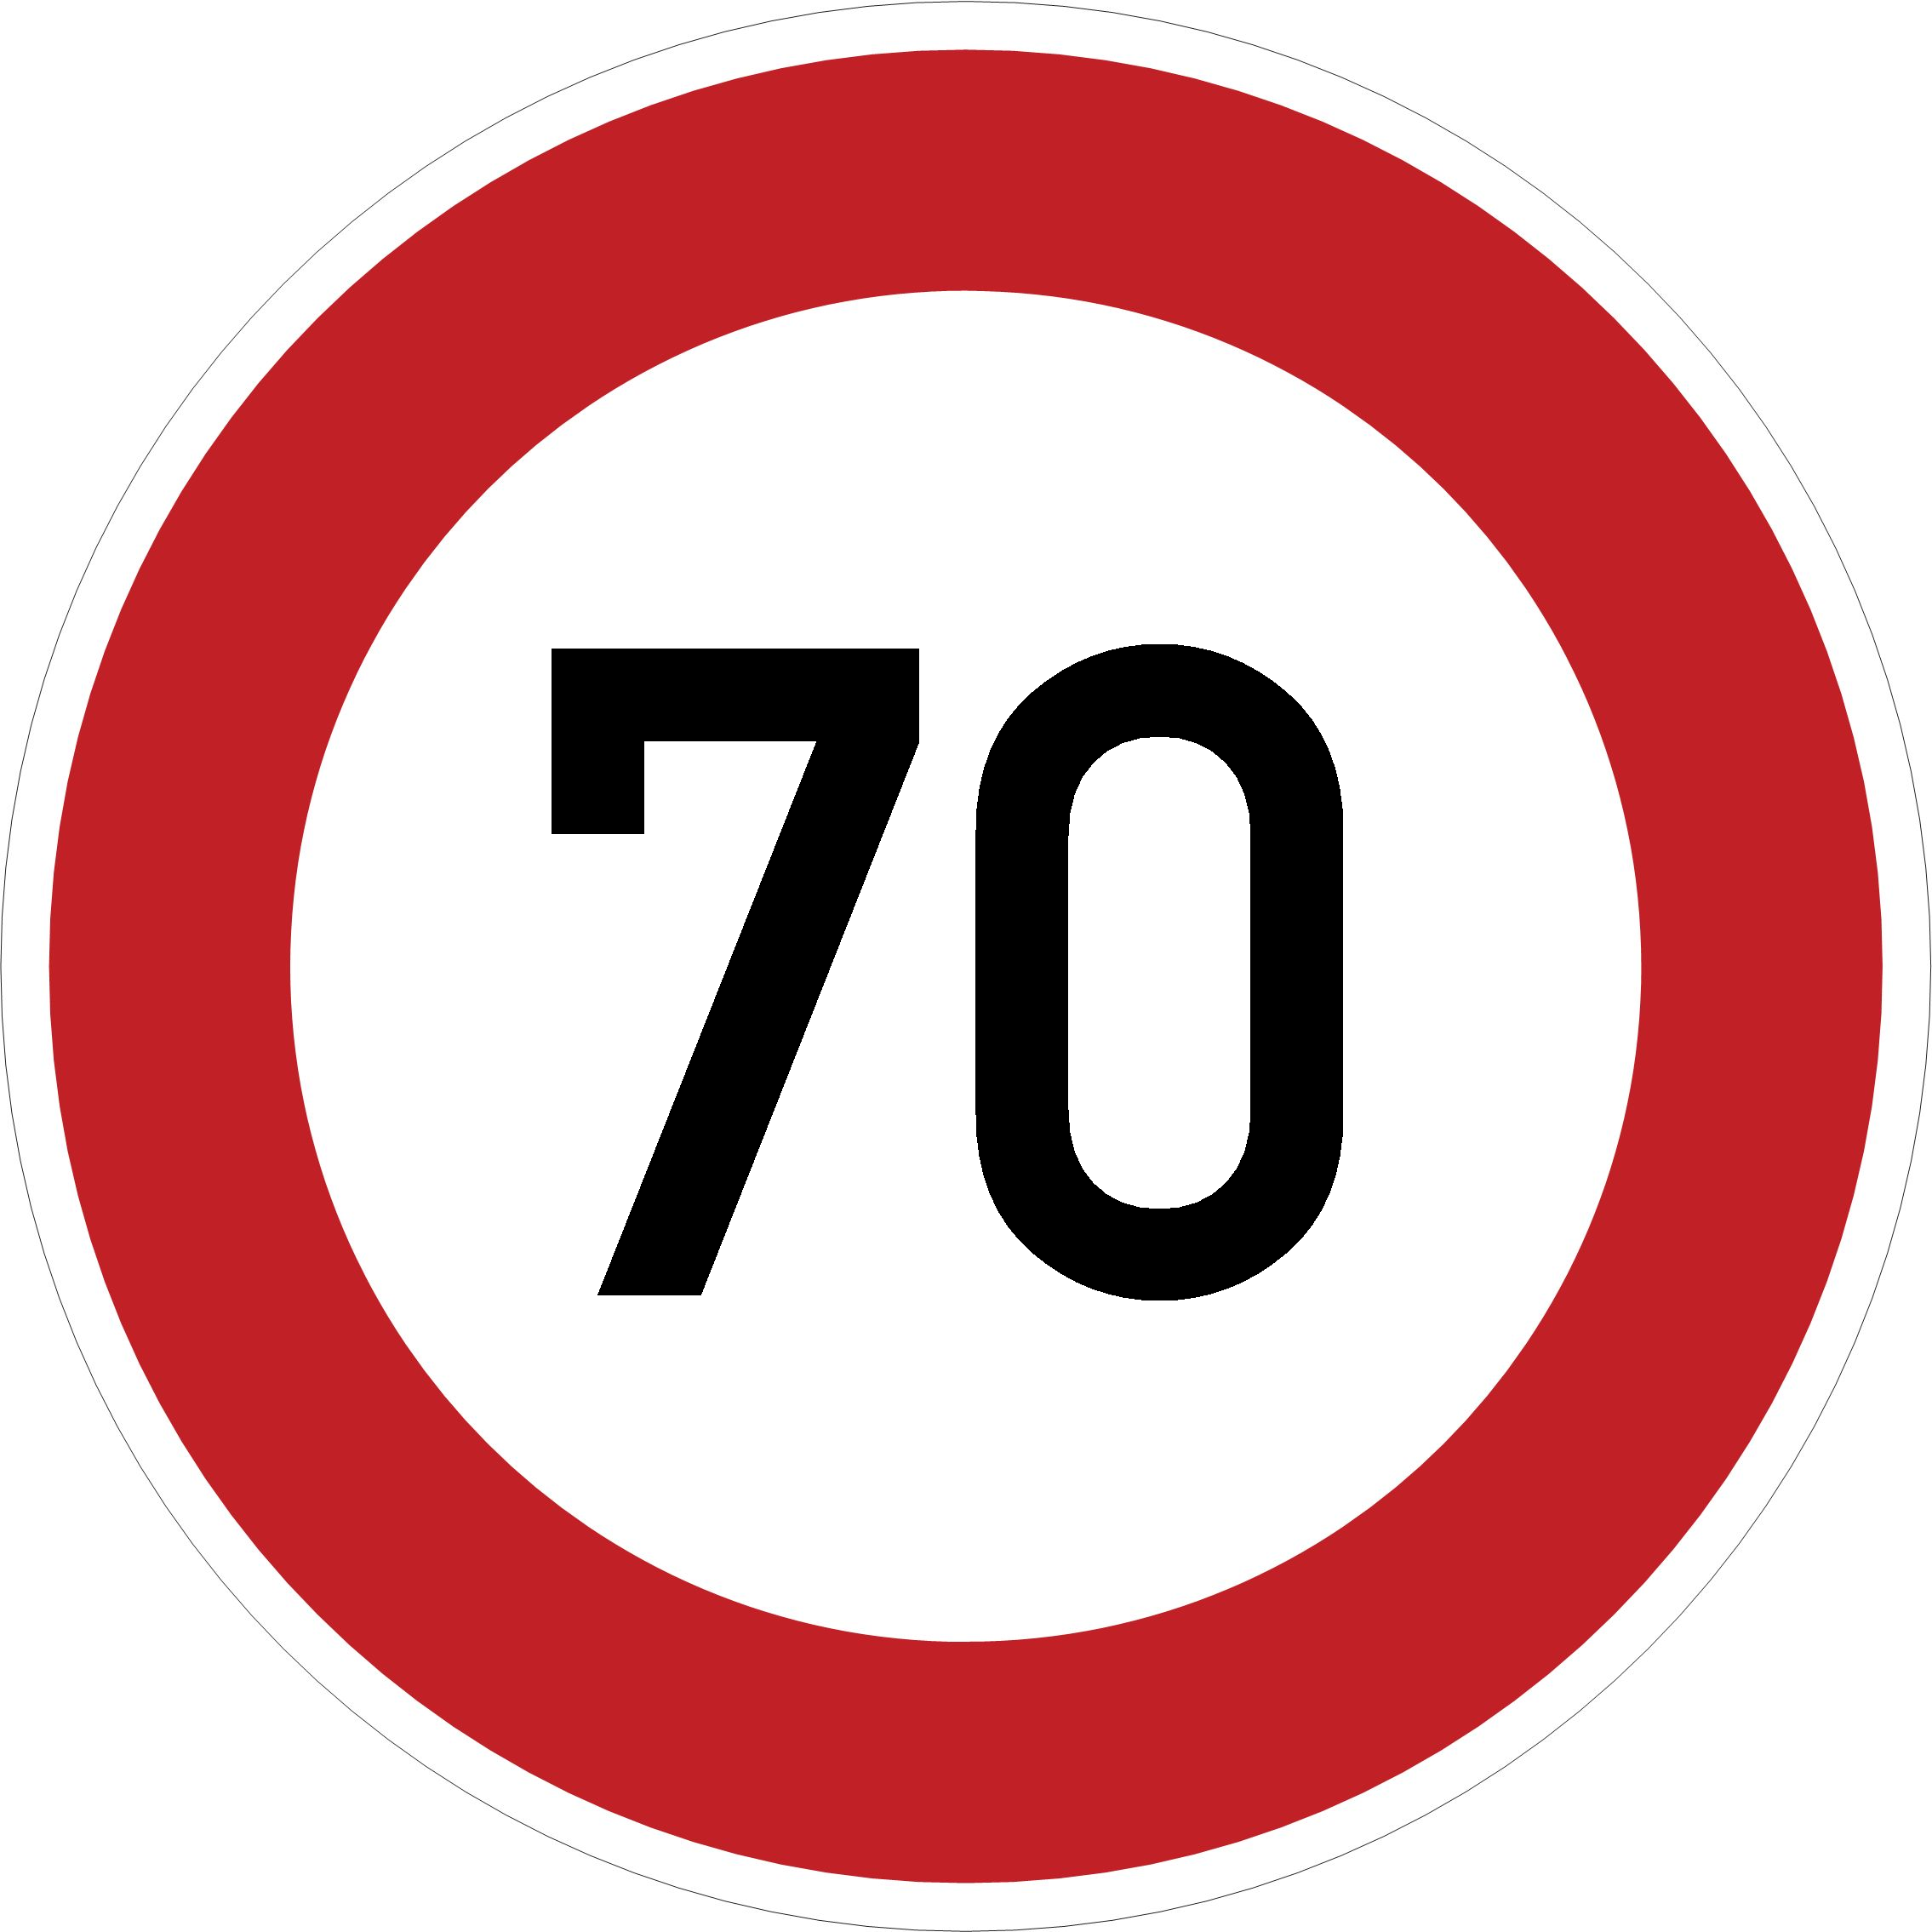
\includegraphics[scale=0.06]{images/70.png}
		\caption{Zul\"assige H\"ochstgeschw.}
		\label{fig:PED}
	\end{minipage}
	\hfill
	\begin{minipage}[t]{10cm}
		\vspace{0pt}
		\begin{itemize}
			\item Der gr\"un markierte Bereich im Zustandsautomaten beschreibt, was das Schild \glqq Zul\"assige H\"ochstgeschwindigkeit 70km/h\grqq \ bewirkt.
			
			\item Wenn als Eingabe \textbf{\textit{70}} empfangen wird, wird das Geschwindigkeitsereignis \textbf{\textit{high}} ver\"offentlicht.
			
			\item Sobald ein Geschwindigkeitsereignis au\ss{}er \textbf{\textit{70}} empfangen wird schaltet der Zustandsautomat zur\"uck auf den Status \textbf{\textit{DEFAULT}}
		\end{itemize}
	\end{minipage}
\end{figure}



	\cleardoublepage
	\section{Fazit und Ausblick}
\label{sec:fazit}
\subsection{Fazit}
\subsubsection{Fazit Rundfahrt}
\subsubsection{Fazit Schildererkennung}
\subsection{Ausblick}
\subsubsection{Ausblick Rundfahrt}
\subsubsection{Ausblick Schildererkennung}
  
	\bibliography{literature}
	\bibliographystyle{alpha}
	
	\begin{appendix}
	\section{Erster Anhang}
	\end{appendix}

\end{document}
